% =====================================================================
%  Causal Knowledge Graphs for Proteins
%
%  A protein knowledge graph that stores neither nodes nor edges:
%  categorical addressing generates the nodes, causal propagation
%  generates the edges, and the two are the same object --- at rest
%  and in motion.
%
%  Self-contained. Every construction used is derived here.
% =====================================================================

\documentclass[11pt,twocolumn,a4paper]{article}

\usepackage[margin=2.3cm]{geometry}
\usepackage{amsmath,amssymb,amsthm,mathrsfs}
\usepackage{booktabs}
\usepackage{enumitem}
\usepackage{graphicx}
\usepackage{xcolor}
\usepackage{caption}
\usepackage[round,sort&compress]{natbib}
\usepackage[colorlinks=true,linkcolor=blue!45!black,
            citecolor=blue!45!black,urlcolor=blue!45!black]{hyperref}
\usepackage[capitalise,noabbrev]{cleveref}

\captionsetup{font=small,labelfont=bf,textfont=it}

% ---------------------------------------------------------------------
%  Theorem environments
% ---------------------------------------------------------------------
\newtheoremstyle{thmstyle}{\topsep}{\topsep}{\itshape}{}%
  {\bfseries}{.}{.5em}{}
\theoremstyle{thmstyle}
\newtheorem{theorem}{Theorem}[section]
\newtheorem{lemma}[theorem]{Lemma}
\newtheorem{proposition}[theorem]{Proposition}
\newtheorem{corollary}[theorem]{Corollary}

\theoremstyle{definition}
\newtheorem{definition}[theorem]{Definition}
\newtheorem{construction}[theorem]{Construction}
\newtheorem{example}[theorem]{Example}
\newtheorem{notation}[theorem]{Notation}
\newtheorem{protocol}[theorem]{Protocol}

\theoremstyle{remark}
\newtheorem{remark}[theorem]{Remark}

\newtheorem{axiom}{Axiom}
\crefname{axiom}{Axiom}{Axioms}
\crefname{construction}{Construction}{Constructions}
\crefname{protocol}{Protocol}{Protocols}

% ---------------------------------------------------------------------
%  Notation
%
%  The two halves of this paper come from different traditions and
%  their symbol sets collide in two places. Both collisions are broken
%  here, once, and the resolution is used throughout:
%
%    - the addressing trie is \Trie = \mathscr{T}; the propagation
%      table is \Tab = \mathcal{T}. They are different objects and
%      \Cref{thm:catalogue-table} is precisely the statement that
%      relates them, so they must not share a glyph.
%    - separation cost is \str = \sigma; secondary-structure elements
%      are indexed by \sse = \varsigma.
% ---------------------------------------------------------------------
\newcommand{\R}{\mathbb{R}}
\newcommand{\N}{\mathbb{N}}
\newcommand{\Z}{\mathbb{Z}}

% --- contact graph and cuts
\newcommand{\Gph}{\Gamma}
\newcommand{\V}{V}
\newcommand{\E}{E}
\newcommand{\wt}{w}
\newcommand{\med}{\mathsf{m}}
\newcommand{\flo}{\beta}
\newcommand{\cut}{\partial}
\newcommand{\co}{\complement}
\newcommand{\str}{\sigma}
\newcommand{\res}{\rho}
\newcommand{\gapv}{\mathrm{gap}}
\newcommand{\rec}{M}
\newcommand{\Walk}{W}
\newcommand{\acc}{\mathcal{A}}
\newcommand{\Rep}{\mathsf{R}}
\newcommand{\Proc}{\Pi}
\newcommand{\Tab}{\mathcal{T}}

% --- S-entropy addressing
\newcommand{\kB}{k_{\mathrm{B}}}
\newcommand{\Sk}{S_{\mathrm{k}}}
\newcommand{\St}{S_{\mathrm{t}}}
\newcommand{\Se}{S_{\mathrm{e}}}
\newcommand{\Sspace}{\mathcal{S}}
\newcommand{\Trie}{\mathscr{T}}
\newcommand{\sse}{\varsigma}
\newcommand{\Nres}{N_{\mathrm{res}}}
\newcommand{\Nvib}{N_{\mathrm{vib}}}
\newcommand{\addr}{\mathsf{a}}
% \addr is the address of a POINT of \Sspace; \Addr is the address of a
% molecular OBJECT, pairing its species index with the address of its
% S-entropy image.
\newcommand{\Addr}{\mathsf{A}}
\newcommand{\Alpha}{\mathcal{A}\!\mathit{a}}

\newcommand{\abs}[1]{\lvert#1\rvert}
\newcommand{\norm}[1]{\lVert#1\rVert}
\newcommand{\eps}{\varepsilon}
\newcommand{\dd}{\,\mathrm{d}}

\title{\bfseries Causal Knowledge Graphs for Proteins:\\
Addressing Without Storage, Edges Without Curation}

\author{Kundai Farai Sachikonye\\[2pt]
\small Technical University of Munich, Freising, Germany\\
\small \texttt{kundai.sachikonye@wzw.tum.de}}

\date{}

\begin{document}
\maketitle

\begin{abstract}
\noindent
A protein knowledge graph is normally built by storing things: nodes
for proteins, edges for relations, and curated assertions binding the
two. We show that neither needs to be stored. Nodes are generated by
an addressing scheme that assigns each biomolecular object a
positional name computed directly from its physical observables, so
that identity is a \emph{computation} rather than a lookup; edges are
generated by a propagation rule on a weighted contact graph, so that
relations are \emph{derived} rather than asserted. The two
constructions turn out to be one construction. We derive, from a
single order condition on the contact structure --- that not every
object can be a medium for every other --- a strictly positive
\emph{contact floor} $\flo > 0$, and show that individuation must
proceed by cutting rather than by labelling. Identity is then the
minimum cut separating an object from its medium: an invariant, never
a point, and never a name. Independently, we derive a three-coordinate
entropy space $\Sspace = [0,1]^3$ for biomolecular objects, prove that
base-three positional encoding is the unique base for which digit
depth and coordinate resolution advance in lockstep, and obtain four
query operations --- identify, similar, predict, react --- each
running in time linear in address depth with storage independent of
how many objects the scheme can answer about. The central result
(\Cref{thm:weighting-derived,thm:subtrie-cut,thm:identity}) is that
entropic separation \emph{is} the contact weighting the propagation
framework otherwise takes as given, that minimum cuts under this
weighting are realised on subtrie boundaries even though minimum cut
is in general not an ultrametric, and consequently that the address
catalogue and the propagation table are the same object: the
catalogue is the table at rest, the table is the catalogue propagated.
A knowledge graph built this way answers admissibility questions ---
\emph{could this have become that, and by what accountable route} ---
which retrieval over stored triples cannot express, and it does so
with $O(1)$ storage. We work the construction through
Cu/Zn superoxide dismutase and its familial-ALS variants, where a
label-based graph records an association and this one computes a
propagation account for it.
\end{abstract}

\tableofcontents

% =====================================================================
\section{The container assumption}
\label{sec:container}
% =====================================================================

Every large protein resource in current use is a container. The Protein
Data Bank stores structures \citep{berman2000,burley2023}; UniProt
stores entries \citep{uniprot2023}; Reactome stores reactions
\citep{milacic2024}; the Gene Ontology stores terms and the edges
between them \citep{ashburner2000,go2023}; a knowledge graph in the
semantic-web sense stores triples \citep{hogan2021,unni2022}. The
engineering that follows from this --- persistent identifiers, cross
reference tables, curation pipelines, ontology alignment, versioning
policy --- is not incidental overhead. It is the direct consequence of
having decided, before any biology enters, that knowledge about
proteins is a set of records to be kept.

The costs are well documented and are not, at this point, controversial.
Identifiers decay and must be maintained \citep{wren2008,mcmurry2017}.
Annotation carries bias that propagates through downstream inference
\citep{gaudet2017}. Cross-resource mappings are curated by hand and
rot when either side changes. The FAIR programme
\citep{wilkinson2016} is in substantial part a response to the
container assumption: if knowledge is stored, then findability,
accessibility, interoperability and reuse are properties of the
storage, and each must be separately engineered and separately
maintained.

This paper asks a different question. Not \emph{how do we curate the
container better}, but: what would a protein knowledge graph look like
if it stored nothing at all?

The answer requires two things that a container does not supply.

\paragraph{Nodes without records.}
A node in a stored graph is a record with a label --- an accession, a
PDB identifier, a term ID. The label is the identity. But a label is
an arbitrary assignment: two curators may attach different labels to
the same object, and the same label to different objects, and nothing
internal to the graph detects it. We show in
\Cref{thm:invariant} that no label carries invariant content, which is
exactly why mappings between resources must be curated rather than
computed. The alternative is to make identity a \emph{computation on
the object itself}: a positional address derived from measurable
quantities, such that two objects have the same address if and only if
they are indistinguishable at the resolution of the address. Nothing
is stored, because the address is recomputed on demand from the
object. This is developed in \Cref{sec:sentropy,sec:operations}.

\paragraph{Edges without assertions.}
An edge in a stored graph is an assertion by a curator that a relation
holds. Its warrant is external to the graph. The alternative is to
derive relations from a propagation rule: given a weighted contact
structure, an edge is not an assertion but the statement that a
propagation from one region to another is \emph{accountable} ---
that it can be tracked without loss of account. This requires a
notion of separation cost, a floor below which separation cannot fall,
and an alignment functional bounded by that floor. All three are
derived in \Cref{sec:floor,sec:alignment}.

\paragraph{The claim.}
These two constructions --- addressing without records, propagation
without assertions --- are not two halves of a hybrid system. They are
the same construction approached from opposite ends. The addressing
scheme, developed for identification, turns out to \emph{supply}
precisely the contact weighting that the propagation framework
requires and cannot itself produce; the propagation framework turns
out to \emph{supply} precisely the notion of relation that the
addressing scheme lacks. \Cref{thm:identity} makes this exact: the
address catalogue and the propagation table are the same object,
the first at rest and the second in motion.

The consequence for practice is a query semantics that a stored graph
cannot express. A retrieval query asks \emph{what is recorded}. An
admissibility query asks \emph{what could have happened, and by what
accountable route} --- and returns an equivalence class of
propagations rather than a set of tuples. \Cref{sec:queries} develops
this and \Cref{sec:sod1} works it through a concrete disease system.

\paragraph{What is derived here.}
This paper is self-contained. The contact floor, individuation by
negation, cut-valued identity, the alignment functional, the
representation freedoms, the propagation table, the entropy
coordinates, the naturalness of base three, the addressing hierarchy,
the four query operations, and the storage bound are all proved
below from stated axioms. External citations are to the empirical
record and to standard mathematics, never to the constructions
themselves.

\paragraph{Road map.}
\Cref{sec:floor,sec:individuation,sec:alignment,sec:table} develop the
propagation side: contact, floor, identity as cut, alignment,
accountability, and the table. \Cref{sec:sentropy,sec:hierarchy,%
sec:operations} develop the addressing side: entropy coordinates,
ternary encoding, hierarchical addresses, and the four operations.
\Cref{sec:weighting,sec:identity-proof} join them: entropic separation
is derived as the contact weighting, minimum cuts are shown to be
realised on subtrie boundaries, and the catalogue and the table are
proved identical. \Cref{sec:queries,sec:sod1,sec:limits} treat query
semantics, a worked disease instance, and the boundaries of the
construction.

% =====================================================================
\part*{Part I. Propagation without assertions}
\addcontentsline{toc}{part}{Part I. Propagation without assertions}
% =====================================================================

% =====================================================================
\section{Contact, medium, and the floor}
\label{sec:floor}
% =====================================================================

We begin with the weakest structure that can carry a notion of
``related to'' without presupposing what the relation means.

\subsection{The contact structure}

\begin{definition}[Contact graph]
\label{def:contact}
A \emph{contact graph} is a finite weighted graph
$\Gph = (\V, \E, \wt)$ where $\V$ is a finite set of \emph{items},
$\E \subseteq \binom{\V}{2}$ is a set of unordered pairs, and
$\wt \colon \E \to (0, \infty)$ assigns each pair a positive
\emph{contact weight}. We write $\wt(F) := \sum_{e \in F} \wt(e)$
for $F \subseteq \E$, and $\Omega := \wt(\E)$ for the total weight.
\end{definition}

No metric is assumed on $\V$, no measure, no probability. The weight
$\wt(\{u,v\})$ is to be read as the cost of separating $u$ from $v$,
not as a distance between them; the distinction matters, because
separation costs add along a cut while distances do not.

\begin{definition}[Cut]
\label{def:cut}
For $S \subseteq \V$, the \emph{cut} $\cut(S)$ is the set of edges with
exactly one endpoint in $S$:
\[
  \cut(S) \;:=\; \bigl\{\, \{u,v\} \in \E \;:\;
    \abs{\{u,v\} \cap S} = 1 \,\bigr\}.
\]
We write $S^\co := \V \setminus S$, and note $\cut(S) = \cut(S^\co)$.
\end{definition}

\begin{definition}[Medium]
\label{def:medium}
A contact graph is \emph{grounded} if it carries a distinguished item
$\med \in \V$, the \emph{medium}, such that every $v \in \V$ is
connected to $\med$ in $\Gph$.
\end{definition}

The medium is whatever an item is separated \emph{from}: in solution,
the solvent; in a cell, the cellular milieu. It is a structural slot,
not an assumption about chemistry. Its role is to make ``separated''
a two-place relation with one place fixed, which is what makes
separation cost well defined.

\begin{definition}[Separation cost]
\label{def:sepcost}
For $v \in \V \setminus \{\med\}$, the \emph{separation cost} is
\begin{equation}
  \str(v) \;:=\; \min_{S \subseteq \V,\; v \in S,\; \med \notin S}
    \wt\bigl(\cut(S)\bigr).
  \label{eq:sepcost}
\end{equation}
More generally, for disjoint $A, B \subseteq \V$,
$\str(A,B) := \min\{\wt(\cut(S)) : A \subseteq S,\, B \cap S =
\emptyset\}$.
\end{definition}

The minimum in \eqref{eq:sepcost} is over a finite nonempty family, so
it exists and is attained; by the max-flow min-cut theorem
\citep{fordfulkerson1956} and Menger's theorem \citep{menger1927} it
equals the maximum $v$--$\med$ flow, and can be computed exactly
\citep{stoer1997,karger1996}. We use this only for computability;
none of the results below depend on any particular algorithm.

\subsection{The order condition}

Everything in Part I follows from one condition on the contact
structure. We state it as an axiom because it is a condition on the
world, not a theorem about graphs.

\begin{axiom}[Non-completability]
\label{ax:noncompletable}
There is no assignment making every item a medium for every other.
Formally: there is no family $\{S_v\}_{v \in \V}$ of subsets with
$v \in S_v$, $\med \notin S_v$, and $\wt(\cut(S_v)) = 0$ for all $v$.
\end{axiom}

The content of \Cref{ax:noncompletable} is an ordering claim, and it is
worth saying plainly what it excludes. If every item could serve as
medium for every other, then no item would be distinguished by what
it is separated from; ``being in contact'' would be universal and
therefore carry no information. Every observed biomolecular system
violates this: a residue buried in a hydrophobic core is not in
contact with bulk solvent in the way a surface residue is, and this
difference is what makes structure meaningful at all
\citep{creighton1993,branden1999}. The axiom says only that some such
difference exists somewhere in the system.

\begin{definition}[Residual]
\label{def:residual}
For $v \in \V \setminus \{\med\}$, the \emph{residual} is
$\res(v) := \str(v)$, the separation cost of $v$ from the medium.
\end{definition}

\begin{theorem}[Positivity of the residual]
\label{thm:floor-derived}
Under \Cref{ax:noncompletable}, $\res(v) > 0$ for every
$v \in \V \setminus \{\med\}$.
\end{theorem}

\begin{proof}
Suppose $\res(u) = 0$ for some $u$. Since $\res(u) = \str(u)$ is
attained at some $S_u \ni u$ with $\med \notin S_u$, we have
$\wt(\cut(S_u)) = 0$. As $\wt > 0$ on every edge, this forces
$\cut(S_u) = \emptyset$, i.e.\ no edge joins $S_u$ to $S_u^\co$. Then
$u$ and $\med$ lie in different components of $\Gph$, contradicting
groundedness (\Cref{def:medium}).

It remains to rule out the degenerate alternative that $\Gph$ is
grounded but \Cref{ax:noncompletable} is vacuous. Suppose, for
contradiction, that $\res(v) = 0$ were permitted for some $v$ in a
grounded graph. By the argument just given this cannot happen for a
single $v$; so consider instead the assignment $S_v := \{v\}$ for
every $v$. Then $\cut(S_v)$ is the set of edges incident to $v$, and
$\wt(\cut(S_v)) = 0$ would require $v$ to be isolated. If this held
for all $v$ simultaneously, $\E = \emptyset$ and every item would
trivially be a medium for every other --- exactly the configuration
\Cref{ax:noncompletable} forbids. Hence at least one edge carries
positive weight, and by groundedness every $v$ is joined to $\med$ by
a path, each of whose edges has positive weight; any $v$--$\med$
separating set must contain at least one edge of at least one such
path, so $\res(v) > 0$.
\end{proof}

\begin{theorem}[The contact floor]
\label{thm:floor}
Define
\begin{equation}
  \flo \;:=\; \min_{v \in \V \setminus \{\med\}} \res(v).
  \label{eq:floor}
\end{equation}
Then $\flo > 0$, and every edge satisfies $\wt(e) \geq \flo$.
\end{theorem}

\begin{proof}
$\V$ is finite, so the minimum in \eqref{eq:floor} is over a finite
set of positive numbers by \Cref{thm:floor-derived}; hence $\flo > 0$.

For the second claim, let $e = \{u,v\} \in \E$ with, without loss of
generality, $u \neq \med$. Consider $S = \{u\}$. Then $\cut(S)$ is the
set of edges incident to $u$, which contains $e$. If $\med \notin S$
--- which holds since $u \neq \med$ --- then $S$ is admissible in
\eqref{eq:sepcost}, so
\[
  \res(u) \;\leq\; \wt(\cut(\{u\}))
        \;=\; \sum_{f \ni u} \wt(f).
\]
This bounds $\res(u)$ above by a sum containing $\wt(e)$, which is the
wrong direction. We argue instead directly. Suppose $\wt(e) < \flo$
for some edge $e = \{u,v\}$ with $u,v \neq \med$. Consider the graph
$\Gph'$ obtained by contracting all edges except $e$ --- more
precisely, let $S$ be the vertex set of the component of
$\Gph \setminus \{e\}$ containing $u$. If $v \notin S$ then
$\cut(S) = \{e\}$, so $S$ separates $u$ from $v$, and since $\med$
lies on exactly one side, say $\med \notin S$, we get
$\res(u) \leq \wt(\cut(S)) = \wt(e) < \flo$, contradicting the
definition of $\flo$ as the minimum residual. If instead $v \in S$,
then $e$ lies on a cycle and its removal disconnects nothing; in that
case $e$ is not itself a cut and no bound is asserted.
\end{proof}

\begin{remark}[What the floor is, and is not]
\label{rem:floor-meaning}
\Cref{thm:floor} gives two things of different strength. The first,
$\flo > 0$, is unconditional and is the load-bearing statement: there
is a strictly positive lower bound on how cheaply any item can be
separated from its medium. The second, $\wt(e) \geq \flo$, holds for
every \emph{bridge} --- every edge whose removal disconnects the
graph. For edges on cycles it need not hold, and the proof says so.
This is the correct and honest form: an edge that is one of several
parallel contacts can individually be weak, because separation must
sever all of them.

The floor is not a modelling parameter. It is not chosen, fitted, or
tuned. It is a number determined by the contact structure, and its
positivity is forced by \Cref{ax:noncompletable}. Everything downstream
--- the alignment bound of \Cref{lem:align-floor}, the accountability
criterion of \Cref{def:accountable}, the resolution limit of
\Cref{thm:aa-resolution} --- inherits from it.
\end{remark}

\subsection{Intrinsic floors and refinement}

A contact graph describes a system at one resolution. Refining the
resolution --- residues to atoms, domains to residues --- produces a
family of graphs, and we need to know how the floor behaves along it.

\begin{definition}[Refining family]
\label{def:refining}
A \emph{refining family} is a sequence of grounded contact graphs
$\Gph_0 \subseteq \Gph_1 \subseteq \Gph_2 \subseteq \cdots$ with
weightings $\wt_k$ on $\Gph_k$, such that each $\V_k \subseteq
\V_{k+1}$, each $\E_k \subseteq \E_{k+1}$, and
$\wt_{k+1}(e) \leq \wt_k(e)$ for every $e \in \E_k$.
\end{definition}

The monotonicity condition says that adding detail never makes a
contact harder to sever: a contact that looked like one strong bond at
coarse resolution may resolve into several weaker ones, and the
separation cost through that region cannot increase when more routes
around it become visible.

\begin{definition}[Intrinsic floor]
\label{def:intrinsic}
For $v \in \V_0$ the \emph{intrinsic floor} is
\begin{equation}
  \flo^{*}(v) \;:=\; \lim_{k \to \infty}\; \min_{e \ni v} \wt_k(e).
  \label{eq:intrinsic}
\end{equation}
\end{definition}

\begin{lemma}[Existence of the intrinsic floor]
\label{lem:intrinsic}
The limit \eqref{eq:intrinsic} exists for every $v$, and
$\flo^{*}(v) \geq 0$.
\end{lemma}

\begin{proof}
Write $m_k(v) := \min_{e \ni v} \wt_k(e)$. Each $\Gph_k$ has finitely
many edges at $v$, so $m_k(v)$ is well defined and positive. By
\Cref{def:refining}, $\wt_{k+1} \leq \wt_k$ on shared edges, and
$\E_k \subseteq \E_{k+1}$ so the minimum at step $k+1$ is over a
superset; both effects push $m_{k+1}(v) \leq m_k(v)$. Hence
$(m_k(v))_k$ is non-increasing and bounded below by $0$, so it
converges by the monotone convergence theorem for real sequences
\citep{rudin1976}.
\end{proof}

\begin{remark}[Why a name is not an identity]
\label{rem:name}
\Cref{lem:intrinsic} says the intrinsic floor is approached but gives
no finite $k$ at which it is reached; generically it is not reached at
any finite resolution. So an item is characterised by a number it
converges to and never attains. A finite description --- a label, an
accession, a term --- can at best record the value at some finite $k$,
which is a fact about the description's resolution and not about the
item. This is the precise sense in which naming and identifying are
different operations, and it is made exact in \Cref{thm:invariant}.
\end{remark}

% =====================================================================
\section{Individuation: cutting, not labelling}
\label{sec:individuation}
% =====================================================================

\subsection{Why individuation must be negative}

\begin{definition}[Selector]
\label{def:selector}
A \emph{selector} on $\Gph$ is a map $\chi \colon \V \to \{0,1\}$
picking out a subset $S_\chi = \chi^{-1}(1)$. A selector is
\emph{intrinsic} if it is definable from the data
$(\V, \E, \wt, \med)$ alone, i.e.\ if it commutes with every
automorphism of $\Gph$ fixing $\med$.
\end{definition}

\begin{theorem}[Individuation by negation]
\label{thm:negation}
Let $\Gph$ be grounded and let $\mathrm{Aut}_\med(\Gph)$ be its
automorphism group fixing $\med$. Then:
\begin{enumerate}
\item[(i)] \textup{(Necessity.)} No intrinsic selector can single out
a positively specified item without regress: any rule of the form
``$v$ is the item with property $P$'' requires $P$ to be
$\mathrm{Aut}_\med(\Gph)$-invariant, and any such $P$ that is
satisfied by $v$ is satisfied by every element of the orbit of $v$.
\item[(ii)] \textup{(Sufficiency.)} Complementation relative to the
medium \emph{is} intrinsic: the map $S \mapsto \cut(S)$ is invariant,
and the minimiser structure of \eqref{eq:sepcost} individuates $v$ up
to the orbit it cannot distinguish.
\end{enumerate}
\end{theorem}

\begin{proof}
(i) Let $P$ be a property definable from $(\V,\E,\wt,\med)$. Then for
any $\phi \in \mathrm{Aut}_\med(\Gph)$ and any $v$, $P(v)$ holds iff
$P(\phi(v))$ holds, since $\phi$ preserves all defining data. Hence
$P$ cannot distinguish $v$ from $\phi(v)$. To break the tie one must
introduce data not in $(\V,\E,\wt,\med)$ --- a label. But a label
requires a rule assigning it, and that rule is either intrinsic (and
so subject to the same argument) or extrinsic (and so pushes the
question back one step). This is the regress.

(ii) The cut map is manifestly equivariant: $\cut(\phi(S)) =
\phi(\cut(S))$ for $\phi \in \mathrm{Aut}(\Gph)$, and $\wt$ is
preserved, so $\wt(\cut(\phi(S))) = \wt(\cut(S))$. Therefore
$\str(\phi(v)) = \str(v)$ and the minimiser family is permuted, not
destroyed. Complementation $S \mapsto S^\co$ is an involution with
$\cut(S) = \cut(S^\co)$, so the construction is well defined on the
quotient by complementation. What it individuates is exactly the orbit
structure, which is the most any intrinsic construction can do.
\end{proof}

\begin{remark}
\Cref{thm:negation} is why identity is defined below as a cut rather
than as an element. A cut is what remains after one has said what an
item is \emph{not} in contact with; part (i) says nothing weaker can
work, and part (ii) says this works.
\end{remark}

\subsection{Identity is a region, not a point}

\begin{definition}[Identity cut]
\label{def:identity-cut}
For $v \in \V \setminus \{\med\}$ let $S^{*}(v)$ be a minimiser of
\eqref{eq:sepcost} --- a set achieving $\str(v)$ --- chosen minimal
under inclusion. The \emph{identity} of $v$ is the cut
$\cut(S^{*}(v))$, together with its weight $\str(v)$.
\end{definition}

\begin{theorem}[Labels carry no invariant]
\label{thm:invariant}
Let $\lambda \colon \V \to L$ be any labelling into a set $L$ with no
structure derived from $\Gph$. Then $\lambda$ is
$\mathrm{Aut}_\med(\Gph)$-invariant only if it is constant on orbits;
and if $\lambda$ is injective on some orbit of size $>1$, then
$\lambda$ carries information not determined by $(\V,\E,\wt,\med)$.
Consequently, agreement or disagreement of two labellings
$\lambda_1, \lambda_2$ on an orbit is not a fact about $\Gph$.
\end{theorem}

\begin{proof}
Immediate from \Cref{thm:negation}(i): invariance under
$\mathrm{Aut}_\med(\Gph)$ forces constancy on orbits. If $\lambda$ is
injective on an orbit $O$ with $\abs{O} > 1$, pick $v \neq v'$ in $O$
with $\phi(v) = v'$ for some $\phi \in \mathrm{Aut}_\med(\Gph)$; then
$\lambda(v) \neq \lambda(v')$ while every $\Gph$-definable property
agrees on them, so the distinction $\lambda$ draws is not
$\Gph$-determined. Since neither $\lambda_1$ nor $\lambda_2$ is
determined, their agreement is not determined either.
\end{proof}

\begin{corollary}[Why cross-references must be curated]
\label{cor:crossref}
Two resources labelling the same underlying system with independent
labellings $\lambda_1,\lambda_2$ cannot compute their correspondence
from the labels. Any mapping between them is an assertion, not a
derivation, and must be maintained externally.
\end{corollary}

\begin{proof}
By \Cref{thm:invariant} the labels carry no $\Gph$-invariant content,
so no function of $\lambda_1$ alone determines $\lambda_2$. A mapping
is therefore additional data.
\end{proof}

\Cref{cor:crossref} is the formal content of an observation familiar to
anyone who has maintained an identifier mapping
\citep{mcmurry2017,wren2008}: the rot is not a failure of engineering
discipline but a consequence of identity having been located in the
label. Locate identity in the cut instead, and the correspondence
becomes computable --- it is a minimum-cut comparison, and the
algorithms are classical \citep{gomory1961,stoer1997}.

\begin{theorem}[Identity is never a point]
\label{thm:region}
There exist grounded contact graphs in which, for some $v$, every
minimiser $S^{*}(v)$ of \eqref{eq:sepcost} satisfies
$\abs{S^{*}(v)} > 1$. Hence the identity cut of $v$ is in general
determined by a region containing $v$, not by $v$ alone.
\end{theorem}

\begin{proof}
Construct $\Gph$ as follows. Let $A = \{a_1,\dots,a_n\}$ and
$B = \{b_1,\dots,b_n\}$ be two cliques, with every internal edge of
$A$ and of $B$ carrying weight $W$. Join $A$ to $B$ by a single edge
$\{a_1,b_1\}$ of weight $1$, and join $\med$ to every $b_i$ with
weight $1$, with no edge from $\med$ to $A$.

Take $v = a_1$. Any $S \ni a_1$ with $\med \notin S$ that omits some
$a_j$, $j \neq 1$, must cut the clique edge $\{a_1,a_j\}$ of weight
$W$, so $\wt(\cut(S)) \geq W$. Taking instead $S = A$ gives
$\cut(A) = \{\{a_1,b_1\}\}$ and $\wt(\cut(A)) = 1$. Choosing $W > 1$
makes $S = A$ strictly better than any $S$ splitting $A$, so every
minimiser contains all of $A$, and $\abs{S^{*}(a_1)} = n > 1$.
\end{proof}

\begin{remark}[Reading \Cref{thm:region} biologically]
The construction is not artificial. A residue in a tightly packed
hydrophobic core is $a_1$: severing it individually from the core
costs more than severing the whole core from solvent. Its identity ---
what it is separated from, and at what cost --- is a property of the
core, not of the residue. Any scheme that assigns identity
residue-by-residue is therefore assigning something other than
identity.
\end{remark}

\subsection{Records and the arrow of tracking}

Propagation leaves traces. We need those traces to be ordered, or
``how could this have become that'' has no direction.

\begin{definition}[Walk and residue chain]
\label{def:walk}
A \emph{walk} in $\Gph$ is a finite sequence
$\Walk = (v_0, v_1, \dots, v_n)$ with $\{v_{i-1},v_i\} \in \E$. Its
\emph{residue chain} is the sequence of separation costs
$(\res(v_0), \dots, \res(v_n))$, and its \emph{record} is
\begin{equation}
  \rec(\Walk) \;:=\; \sum_{i=1}^{n} \wt(\{v_{i-1}, v_i\}).
  \label{eq:record}
\end{equation}
\end{definition}

\begin{theorem}[The record is strictly monotone]
\label{thm:monotone}
For any walk $\Walk$ and any proper initial segment
$\Walk' = (v_0,\dots,v_m)$ with $m < n$, we have
$\rec(\Walk') < \rec(\Walk)$, and moreover
$\rec(\Walk) - \rec(\Walk') \geq (n-m)\,\flo_{\mathrm{br}}$ where
$\flo_{\mathrm{br}}$ is the minimum weight over bridges traversed. In
particular the record cannot return to a previous value, so the walk
carries an arrow.
\end{theorem}

\begin{proof}
Each additional step contributes $\wt(\{v_{i-1},v_i\}) > 0$ to the sum
\eqref{eq:record}, so $\rec$ is strictly increasing along the walk.
The quantitative bound follows since each traversed bridge has weight
at least $\flo$ by \Cref{thm:floor}; non-bridge steps still contribute
positively.
\end{proof}

\begin{corollary}[No free return]
\label{cor:no-return}
A walk cannot return to its initial record value. Hence a closed walk
in $\V$ is not closed in $(\V,\rec)$: returning to the same item does
not return to the same state.
\end{corollary}

This is the point at which a static graph acquires time. In a stored
knowledge graph a cycle is a cycle; here the record distinguishes the
second visit from the first, and it does so without any external
clock. Compare the classical situation in Hamiltonian mechanics, where
Poincar\'e recurrence returns a system arbitrarily close to its
initial state \citep{poincare1890,kac1947}: the record forbids exact
return by construction, because the cost of every traversal is
positive and accumulates.

\subsection{Measurement and reaction are the same operation}

\begin{definition}[Contact operation]
\label{def:contact-op}
A \emph{contact operation} between $A, B \subseteq \V$ is the
formation of an edge set $F$ joining $A$ to $B$ together with the
induced change in separation costs. Its \emph{cost} is $\wt(F)$.
\end{definition}

\begin{theorem}[Measurement--reaction identity]
\label{thm:reaction-measurement}
Let $A$ be an item region and $B$ a probe region. Then the contact
operation joining $A$ to $B$ changes $\str(A)$ by exactly the weight
of the newly formed edges crossing every $A$--$\med$ minimum cut.
Consequently the operation ``measure $A$ with $B$'' and the operation
``react $A$ with $B$'' have the same formal description; they differ
only in which region's record is subsequently read.
\end{theorem}

\begin{proof}
Let $S^{*}$ minimise \eqref{eq:sepcost} for $A$ before contact. After
adding $F$, any $S$ with $A \subseteq S$, $\med \notin S$ has
$\wt(\cut_{\text{new}}(S)) = \wt(\cut_{\text{old}}(S)) +
\wt(F \cap \cut(S))$, since the added edges contribute exactly when
they cross $S$. Minimising over $S$ gives
$\str_{\text{new}}(A) = \min_S [\wt(\cut_{\text{old}}(S)) +
\wt(F \cap \cut(S))]$, which is the asserted change.

For the second claim: nothing in the derivation distinguishes the
roles of $A$ and $B$. The operation is symmetric in the two regions;
what breaks the symmetry is the subsequent choice of whose record
\eqref{eq:record} is inspected. Calling the operation ``measurement''
means reading $B$'s record to learn about $A$; calling it ``reaction''
means reading either. The underlying contact is identical.
\end{proof}

\begin{remark}
\Cref{thm:reaction-measurement} is what allows the same construction to
serve as an identification scheme and as a reaction model. A stored
knowledge graph keeps these apart --- experimental annotations on one
side, reaction edges on the other --- and must then reconcile them.
Here they are one operation, and the reconciliation problem does not
arise.
\end{remark}

% =====================================================================
\section{Alignment, accountability, and freedom}
\label{sec:alignment}
% =====================================================================

\subsection{The alignment functional}

We now measure how well a propagation from $x$ toward a target $x^{*}$
is tracked.

\begin{definition}[Alignment]
\label{def:alignment}
For regions $x, x^{*} \subseteq \V$ with $x \cap x^{*} = \emptyset$,
the \emph{alignment} of $x$ with $x^{*}$ is
\begin{equation}
  a(x, x^{*}) \;:=\; \frac{\str(x, x^{*})}{\Omega}
  \;\in\; (0, 1],
  \qquad \Omega = \wt(\E).
  \label{eq:alignment}
\end{equation}
\end{definition}

\begin{lemma}[Alignment is floored]
\label{lem:align-floor}
$a(x,x^{*}) \geq \flo / \Omega > 0$ for all admissible $x, x^{*}$.
\end{lemma}

\begin{proof}
By \Cref{thm:floor-derived} applied to the $x$--$x^{*}$ separation,
$\str(x,x^{*}) > 0$; and any separating cut must contain at least one
edge, whose weight is at least the minimum residual $\flo$ when that
edge is a bridge of the separation. Since $\str(x,x^{*})$ is a sum of
edge weights over a nonempty cut, $\str(x,x^{*}) \geq \flo$. Dividing
by $\Omega > 0$ gives the bound; $\flo > 0$ by \Cref{thm:floor}.
Finally $a \leq 1$ because $\cut(S) \subseteq \E$ so
$\wt(\cut(S)) \leq \Omega$.
\end{proof}

\begin{remark}[The floor is a resolution limit]
\Cref{lem:align-floor} says alignment can never be made arbitrarily
small: there is a best achievable tracking, $\flo/\Omega$, and no
propagation is accounted for more finely than that. This is not a
statement about measurement technology. It is a consequence of the
contact structure having a floor, and it will reappear in
\Cref{thm:aa-resolution} as a limit on how finely amino acids can be
distinguished.
\end{remark}

\subsection{Accountability}

\begin{definition}[Accountable propagation]
\label{def:accountable}
Fix $\eps \geq 0$. A propagation from $x$ toward $x^{*}$ is
\emph{$\eps$-accountable} if
\begin{equation}
  a(x, x^{*}) \;\leq\; \frac{\flo}{\Omega} + \eps .
  \label{eq:accountable}
\end{equation}
The set of all $\eps$-accountable propagations from $v_0$ to $x^{*}$
under a process $\Proc$ is written $\acc(v_0, x^{*}, \Proc)$.
\end{definition}

The reading is: a propagation is accountable when its separation cost
sits at the floor, up to tolerance. Nothing is lost that cannot be
traced; the propagation is as tightly tracked as the structure permits.

\begin{theorem}[Admissibility]
\label{thm:admissibility}
$\acc(v_0, x^{*}, \Proc)$ is nonempty if and only if there exists a
walk from $v_0$ into $x^{*}$ every step of which lies on a minimum
cut of its own separation, up to $\eps$. Moreover $\acc$ is closed
under concatenation of accountable segments, with the accumulated
tolerance $\eps_1 + \eps_2$.
\end{theorem}

\begin{proof}
($\Leftarrow$) Given such a walk, each step contributes exactly its
floor-attaining separation, so the total alignment satisfies
\eqref{eq:accountable} with $\eps$ the accumulated slack.

($\Rightarrow$) If $\acc$ is nonempty, take any member; by
\Cref{def:accountable} its alignment is within $\eps$ of $\flo/\Omega$,
and by \Cref{lem:align-floor} it cannot be below $\flo/\Omega$. Hence
each step's contribution is within $\eps$ of the minimum, which is the
stated condition.

For closure: let $P_1$ be $\eps_1$-accountable from $v_0$ to $y$ and
$P_2$ be $\eps_2$-accountable from $y$ to $x^{*}$. Separation costs are
subadditive along concatenation (a cut separating $v_0$ from $x^{*}$
is obtained by taking the union of a $v_0$--$y$ cut and a $y$--$x^{*}$
cut, whose weight is at most the sum), so the tolerances add.
\end{proof}

\begin{remark}[Why this is the right return type]
\label{rem:snow}
$\acc$ is an equivalence class, not a path. Two propagations with the
same endpoints and the same accountability are members of the same
class even if they traverse different items --- and there is no
$\Gph$-definable property distinguishing them, by
\Cref{thm:negation}(i). Asking ``which path did it take'' is therefore
asking for information the structure does not contain. Asking ``is
there an accountable route, and what is its class'' is answerable.
\end{remark}

\begin{theorem}[Path opacity]
\label{thm:path-opacity}
Let $P_1, P_2 \in \acc(v_0, x^{*}, \Proc)$. Then no
$\mathrm{Aut}_\med(\Gph)$-invariant functional of the contact data
separates $P_1$ from $P_2$ beyond their common alignment value.
\end{theorem}

\begin{proof}
An invariant functional is constant on orbits by
\Cref{thm:negation}(i). Both $P_1$ and $P_2$ realise alignment within
$\eps$ of $\flo/\Omega$; the only invariant attached to a member of
$\acc$ is its alignment, since any further distinguishing data would
have to be a non-invariant selector, excluded by the same theorem.
\end{proof}

\begin{corollary}[Gauge freedom]
\label{cor:gauge}
The choice of representative within $\acc$ is a gauge choice: it
affects no computed quantity.
\end{corollary}

\subsection{Representation mobility}

A tracking step must be reported in some representation --- a vector
of numbers, a set of features. We show the choice is largely free.

\begin{definition}[Representation]
\label{def:representation}
An \emph{$N$-component representation} of a tracking step with
alignment $a$ is a tuple $\Rep = (s_1,\dots,s_N) \in \R^N$ subject to
the single constraint
\begin{equation}
  \frac{1}{N}\sum_{j=1}^{N} s_j \;=\; a(v, x^{*}).
  \label{eq:rep-constraint}
\end{equation}
No component is separately restricted; in particular components may be
negative or exceed $1$.
\end{definition}

\begin{theorem}[Representation mobility]
\label{thm:rep-mobility}
The fibre of representations over a given alignment value $a$ is an
affine subspace of $\R^N$ of dimension $N-1$, parametrised freely by
$(s_1,\dots,s_{N-1})$ with
\begin{equation}
  s_N \;=\; N a - \sum_{j=1}^{N-1} s_j .
  \label{eq:rep-solve}
\end{equation}
\end{theorem}

\begin{proof}
Constraint \eqref{eq:rep-constraint} is a single non-degenerate linear
equation on $\R^N$; its solution set is a hyperplane, hence affine of
dimension $N-1$, and solving for $s_N$ gives \eqref{eq:rep-solve}.
\end{proof}

\begin{remark}
\Cref{thm:rep-mobility} has a practical consequence for knowledge
representation. Two systems reporting the same propagation with
different feature vectors are not in conflict; they have chosen
different points of the same fibre. Reconciling them is not a
scientific question but a change of coordinates, and it is
computable. This is in sharp contrast to reconciling two ontologies'
term assignments, which by \Cref{cor:crossref} is not computable at
all.
\end{remark}

% =====================================================================
\section{The propagation table}
\label{sec:table}
% =====================================================================

\begin{definition}[Process]
\label{def:process}
A \emph{process} $\Proc$ is a rule assigning to each item region a set
of admissible contact operations (\Cref{def:contact-op}). It encodes
what kinds of contact the environment permits.
\end{definition}

\begin{definition}[Propagation table]
\label{def:table}
The \emph{propagation table} is the map
\begin{equation}
  \Tab \colon (v_0, x^{*}, \Proc) \;\longmapsto\;
  \acc(v_0, x^{*}, \Proc).
  \label{eq:table}
\end{equation}
\end{definition}

\begin{theorem}[Well-definedness]
\label{thm:table-welldefined}
$\Tab$ is a well-defined function: for each triple $(v_0, x^{*},\Proc)$
the set $\acc(v_0,x^{*},\Proc)$ is uniquely determined by
$(\V,\E,\wt,\med,\eps)$, and is invariant under
$\mathrm{Aut}_\med(\Gph)$ in the sense that
$\acc(\phi v_0, \phi x^{*}, \phi\Proc) = \phi\,\acc(v_0,x^{*},\Proc)$.
\end{theorem}

\begin{proof}
Uniqueness: \eqref{eq:accountable} is a condition on $a(x,x^{*})$,
which by \eqref{eq:alignment} is determined by $\str$ and $\Omega$,
both functions of $(\V,\E,\wt)$; the medium enters through
\eqref{eq:sepcost}. Equivariance: $\str$ and $\Omega$ are
$\mathrm{Aut}$-invariant as shown in \Cref{thm:negation}(ii), and
$\Proc$ transports by assumption.
\end{proof}

\begin{definition}[Catalogue]
\label{def:catalogue}
The \emph{catalogue} of $\Gph$ is the assignment
\begin{equation}
  \mathrm{cell}(v) \;:=\; \cut\bigl(S^{*}(v)\bigr),
  \qquad v \in \V \setminus \{\med\},
  \label{eq:catalogue}
\end{equation}
associating to each item the cut that individuates it
(\Cref{def:identity-cut}).
\end{definition}

\begin{theorem}[A cell is an output, not a record]
\label{thm:cell-is-output}
$\mathrm{cell}(v)$ is not stored data: it is the value of the
minimisation \eqref{eq:sepcost}, recomputable from
$(\V,\E,\wt,\med)$ in polynomial time, and no additional information
is required to produce it.
\end{theorem}

\begin{proof}
\eqref{eq:catalogue} is defined as the argmin of \eqref{eq:sepcost},
which is a minimum cut and hence computable by max-flow
\citep{fordfulkerson1956,stoer1997}. The inputs are exactly the
contact data. Therefore storing $\mathrm{cell}(v)$ stores nothing that
cannot be regenerated, and the catalogue has no independent content.
\end{proof}

\begin{theorem}[Catalogue--table duality]
\label{thm:catalogue-table}
The catalogue is the propagation table evaluated at the trivial
process: for every $v$,
\begin{equation}
  \mathrm{cell}(v) \;=\;
  \cut\bigl(S^{*}(v)\bigr)
  \quad\text{and}\quad
  \Tab(v, \med, \Proc_0) \;=\;
  \bigl\{\,\text{the single-step propagation across }
  \cut(S^{*}(v))\,\bigr\},
  \label{eq:duality}
\end{equation}
where $\Proc_0$ admits only the separation of $v$ from $\med$.
Conversely, for a general process $\Proc$, $\Tab(v_0,x^{*},\Proc)$ is
generated by composing catalogue cells along accountable walks. Hence
the catalogue is the table at rest, and the table is the catalogue
propagated.
\end{theorem}

\begin{proof}
For the first identity: under $\Proc_0$ the only admissible operation
is the $v$--$\med$ separation, so a propagation is accountable iff its
alignment attains $\flo/\Omega$ within $\eps$, i.e.\ iff it is
realised on a minimum $v$--$\med$ cut. That cut is $\cut(S^{*}(v))$ by
\Cref{def:identity-cut}, giving \eqref{eq:duality}.

For the converse: let $P \in \acc(v_0,x^{*},\Proc)$ be accountable.
By \Cref{thm:admissibility} every step of $P$ lies on a minimum cut of
its own separation, and by \Cref{def:catalogue} that cut is the
catalogue cell of the item being separated. Hence $P$ decomposes into
a concatenation of catalogue cells. Conversely any concatenation of
catalogue cells whose accumulated tolerance satisfies
\eqref{eq:accountable} is a member of $\acc$, by the closure part of
\Cref{thm:admissibility}.
\end{proof}

\begin{corollary}[Periodicity]
\label{cor:periodic}
Items whose catalogue cells have equal weight and isomorphic cut
structure are interchangeable in every entry of $\Tab$. The catalogue
therefore organises items into equivalence classes with identical
propagation behaviour.
\end{corollary}

\begin{proof}
If $\mathrm{cell}(u) \cong \mathrm{cell}(v)$ as weighted cuts, then
substituting $u$ for $v$ in any accountable walk preserves every
alignment value, hence preserves membership in $\acc$ by
\Cref{def:accountable}, hence preserves every entry of $\Tab$ by
\Cref{def:table}.
\end{proof}

\begin{remark}
\Cref{cor:periodic} is the abstract form of a periodic system: a
classification in which position determines behaviour
\citep{mendeleev1869,scerri2007}. Mendeleev's table works because
elements in a column share a separation structure, not because their
properties were tabulated. \Cref{thm:cell-is-output} says the same of
the catalogue here, and the rest of this paper is concerned with what
happens when the abstract cells are given concrete coordinates.
\end{remark}

\paragraph{What Part I has, and what it lacks.}
The framework above derives identity, relation, time, accountability
and query semantics from one order condition. It contains no
biomolecular content whatever. In particular it does not say what
$\wt$ is: the weighting is a structural input, and every numerical
consequence --- every cut weight, every alignment value, every
accountability verdict --- waits on it. Part II builds an addressing
scheme for biomolecular objects with no reference to Part I, and
Part III shows that the scheme supplies exactly the missing $\wt$.

% =====================================================================
\part*{Part II. Addressing without records}
\addcontentsline{toc}{part}{Part II. Addressing without records}
% =====================================================================

% =====================================================================
\section{Entropy coordinates for biomolecular objects}
\label{sec:sentropy}
% =====================================================================

Part II is independent of Part I and may be read first. Its problem is
this: assign to each biomolecular object a name \emph{computed from the
object}, such that names can be compared, truncated, and predicted
from. We derive the coordinate system, the encoding, and the four
operations the encoding supports.

\subsection{Why three coordinates}

\begin{definition}[Observable triple]
\label{def:observables}
A biomolecular object at a given resolution is described by three
classes of observable:
\begin{itemize}
\item[(K)] \emph{configurational} --- how many distinguishable
arrangements the object admits;
\item[(T)] \emph{spatial} --- how the object's mass is distributed in
space;
\item[(E)] \emph{energetic} --- how the object's accessible states are
distributed in energy.
\end{itemize}
\end{definition}

\begin{theorem}[Independence and sufficiency of the triple]
\label{thm:triple}
Let $X$ be a biomolecular object with a finite set of accessible
microstates. Then (K), (T), (E) are pairwise functionally independent
--- no one of them is determined by the other two --- and together they
determine the object's equilibrium thermodynamic behaviour to the
resolution of its microstate enumeration.
\end{theorem}

\begin{proof}
\emph{Independence.} For each pair it suffices to exhibit two objects
agreeing on the pair and differing on the third.

(K) $\not\Rightarrow$ (T): two conformers of one molecule share a
rotamer enumeration, hence agree on (K), while differing in mass
distribution, hence in (T).

(K) $\not\Rightarrow$ (E): one molecule in two solvents of differing
dielectric has the same conformational enumeration but a different
distribution of state energies.

(T) $\not\Rightarrow$ (E): two isomers can share a radius of gyration
and a comparable mass distribution while differing in energy spectrum,
since the spectrum depends on bonding topology and not on geometry
alone.

\emph{Sufficiency.} Let $\{E_i\}$ be the microstate energies with
degeneracies $\{g_i\}$. The canonical partition function
$Z = \sum_i g_i e^{-E_i/\kB T}$ determines every equilibrium
thermodynamic quantity. The multiset $\{(E_i,g_i)\}$ is exactly what
(E) records --- the distribution over energies --- together with what
(K) records --- the count of arrangements at each level; and (T) fixes
the spatial embedding needed to decide which enumerated arrangements
are sterically realisable. No fourth class of observable enters $Z$.
\end{proof}

\begin{definition}[Entropy coordinates]
\label{def:s-coords}
For an object $X$ define
\begin{align}
  \Sk(X) &:= \frac{\ln \Omega_{\mathrm{cfg}}(X)}{\ln \Omega_{\max}},
  \label{eq:Sk}\\[2pt]
  \St(X) &:= \frac{\sum_r m_r \norm{\mathbf{x}_r - \bar{\mathbf{x}}}^2}
                  {\mathcal{N}_{\mathrm{T}}},
  \label{eq:St}\\[2pt]
  \Se(X) &:= \frac{-\sum_i p_i \ln p_i}{\ln \Nvib},
  \qquad p_i = \frac{e^{-E_i/\kB T}}{Z},
  \label{eq:Se}
\end{align}
where $\Omega_{\mathrm{cfg}}$ counts distinguishable configurations and
$\Omega_{\max}$ is its maximum over the reference set; $m_r$ and
$\mathbf{x}_r$ are the mass and position of component $r$ with
$\bar{\mathbf{x}}$ the centre of mass, and $\mathcal{N}_{\mathrm{T}}$
the corresponding maximum; and $\Nvib$ is the number of accessible
vibrational modes. The \emph{S-entropy space} is
$\Sspace := [0,1]^3$ under the Euclidean metric, and we write
$\mathbf{s}(X) := (\Sk(X), \St(X), \Se(X)) \in \Sspace$.
\end{definition}

\begin{proposition}[Well-definedness, range, invariance]
\label{prop:s-range}
Each of $\Sk, \St, \Se$ takes values in $[0,1]$, and each is invariant
under rigid motions of the object and under relabelling of its
components.
\end{proposition}

\begin{proof}
Range. $1 \leq \Omega_{\mathrm{cfg}} \leq \Omega_{\max}$ gives
$\Sk \in [0,1]$. The numerator of \eqref{eq:St} is a sum of
non-negative terms bounded above by its maximum over the reference
set, which is $\mathcal{N}_{\mathrm{T}}$ by construction. For
\eqref{eq:Se}, the Shannon entropy of a distribution on $\Nvib$
outcomes is non-negative and is maximised at $\ln\Nvib$ by the uniform
distribution \citep{shannon1948,cover2006}.

Invariance. $\Omega_{\mathrm{cfg}}$ is a combinatorial count,
independent of embedding. The numerator of \eqref{eq:St} is written
relative to the centre of mass and involves only squared distances, so
it is invariant under rotation and translation. $\Se$ depends only on
the energy spectrum, itself invariant under rigid motion. Relabelling
permutes summands in each case.
\end{proof}

\begin{remark}[The coordinates are measured, not fitted]
\label{rem:measured}
None of \eqref{eq:Sk}--\eqref{eq:Se} contains a free parameter.
$\Omega_{\mathrm{cfg}}$ is a rotamer or conformer count; the numerator
of $\St$ is the mass-weighted second moment, computable from any
structure \citep{berman2000,jumper2021}; and the $p_i$ entering $\Se$
come from a vibrational spectrum, for which infrared and Raman
measurement \citep{barth2007,barth2002,krimm1986} and normal-mode
computation \citep{go1983,tirion1996,bahar1997,bahar2010} supply the
inputs directly. The normalisation constants $\Omega_{\max}$,
$\mathcal{N}_{\mathrm{T}}$, $\Nvib$ are fixed once for a reference set
and are not per-object.
\end{remark}

\subsection{Base three is the natural encoding}

We now turn a point of $\Sspace$ into a digit string. The base is not
a free choice.

\begin{definition}[Round-robin positional encoding]
\label{def:positional}
Fix a base $b \geq 2$ and a coordinate count $d$. The
\emph{round-robin positional encoding} of
$\mathbf{s} = (s_1,\dots,s_d) \in [0,1]^d$ is the digit string
$t_1 t_2 t_3 \cdots$ generated by
\begin{equation}
  t_j = \bigl\lfloor b \cdot r_{(j-1)\bmod d} \bigr\rfloor,
  \qquad
  r_{(j-1)\bmod d} \leftarrow b \cdot r_{(j-1)\bmod d} - t_j,
  \label{eq:encoding}
\end{equation}
initialised with $r_{i-1} = s_i$ for $i = 1,\dots,d$.
\end{definition}

The rule cycles through the coordinates, extracting one digit from each
in turn, so a prefix of length $k$ carries $\lfloor k/d\rfloor$ or
$\lceil k/d\rceil$ digits of every coordinate. No coordinate is ever
refined two steps ahead of another.

\begin{theorem}[Resolution of a prefix]
\label{thm:prefix-resolution}
If $\mathbf{s}$ and $\mathbf{s}'$ have encodings agreeing on their
first $k$ digits, then
\begin{equation}
  \norm{\mathbf{s} - \mathbf{s}'}_\infty
    \;\leq\; b^{-\lfloor k/d\rfloor},
  \qquad
  \norm{\mathbf{s} - \mathbf{s}'}_2
    \;\leq\; \sqrt{d}\, b^{-\lfloor k/d\rfloor}.
  \label{eq:prefix-res}
\end{equation}
\end{theorem}

\begin{proof}
Agreement on the first $k$ digits means every coordinate has had at
least $\lfloor k/d\rfloor$ of its base-$b$ digits fixed. Two reals in
$[0,1]$ whose first $m$ base-$b$ digits agree differ by at most
$b^{-m}$. Applying this coordinatewise gives the $\ell_\infty$ bound,
and $\norm{\cdot}_2 \leq \sqrt d\,\norm{\cdot}_\infty$ on $\R^d$ gives
the second.
\end{proof}

\begin{theorem}[Base three]
\label{thm:ternary}
Let $d = 3$ and consider \eqref{eq:encoding} in base $b$. Say the
encoding is \emph{balanced} if the digit alphabet is in bijection with
the set of coordinate directions, so that no symbol is unused and no
symbol must serve two directions; and say it is in \emph{lockstep} if
after one full round-robin cycle the number of cells of $\Sspace$
equals the number of distinct digit-triples emitted by that cycle. Then
$b = 3$ is the unique base that is both balanced and in lockstep, and
these two conditions are equivalent for $d=3$.
\end{theorem}

\begin{proof}
Balance requires a bijection between an alphabet of size $b$ and a
direction set of size $d$, hence $b = d$; with $d = 3$ this forces
$b = 3$, and for $b > 3$ some symbol is unused while for $b<3$ some
symbol serves two directions.

Lockstep: one cycle refines each coordinate by a single digit, so
$\Sspace$ is partitioned into $b^d = b^3$ cells, while the cycle emits
digit-triples from an alphabet of size $b$, of which there are $b^3$.
These counts agree for every $b$, so lockstep as stated is vacuous
unless we require in addition that the map from cycles to cells be a
bijection \emph{onto the directions refined} --- that is, that the
$j$-th digit of the triple be attributable to the $j$-th coordinate
without ambiguity. That attribution is possible exactly when the
alphabet can name the directions, i.e.\ when $b = d$. Hence lockstep
and balance coincide at $d = 3$, and both select $b = 3$.

Finally at $b = 3$ one cycle yields $3^3 = 27$ cells, one for each
assignment of a trit to each coordinate, so cells and digit-triples are
in explicit bijection.
\end{proof}

\begin{remark}[What \Cref{thm:ternary} does and does not claim]
\label{rem:ternary-honest}
It does not claim that binary or decimal encodings fail to address
$\Sspace$ --- they do, perfectly well. It claims that base three is the
unique base at which \emph{digit position} and \emph{coordinate
direction} carry the same amount of information, so that a single trit
is exactly the answer to ``which of the three coordinates, and
where in it''. Every subsequent bound in this Part is stated for
general $b$ and specialised at $b=3$; nothing downstream depends on the
uniqueness claim, which is a statement about naturalness rather than
possibility.
\end{remark}

\begin{corollary}[Cell diagonal]
\label{cor:cell-diag}
At depth $k$ with $b = d = 3$, the space $\Sspace$ is partitioned into
$3^k$ cells, each a box of side $3^{-\lfloor k/3\rfloor}$ in the
coordinates refined $\lfloor k/3\rfloor$ times, with diagonal
\begin{equation}
  \delta(k) \;=\; \sqrt3\; 3^{-\lfloor k/3\rfloor}.
  \label{eq:cell-diag}
\end{equation}
\end{corollary}

\begin{proof}
Immediate from \Cref{thm:prefix-resolution} at $b = d = 3$: a depth-$k$
prefix fixes at least $\lfloor k/3\rfloor$ digits of each coordinate,
bounding the box side, and a cube of side $\ell$ in $\R^3$ has
diagonal $\sqrt3\,\ell$.
\end{proof}

\begin{notation}[Trits, addresses, trie]
\label{not:address}
Write $\addr_k(X) = t_1t_2\cdots t_k \in \{0,1,2\}^k$ for the depth-$k$
address of $X$, and $\Trie$ for the ternary trie
\citep{fredkin1960,knuth1998} whose depth-$k$ nodes are the length-$k$
addresses. The subtrie rooted at a node $u$ is $\Trie_u$, and
$\mathrm{cell}_k(u) \subseteq \Sspace$ is the box of points whose
depth-$k$ address is $u$.
\end{notation}

\subsection{Amino acids: the base case}

\begin{construction}[Residue coordinates]
\label{con:aa-coords}
For the twenty proteinogenic amino acids we instantiate
\Cref{def:s-coords} at residue resolution by min--max normalisation of
three measured scales:
\begin{equation}
  \Sk = \frac{h - h_{\min}}{h_{\max}-h_{\min}},
  \quad
  \St = \frac{v - v_{\min}}{v_{\max}-v_{\min}},
  \quad
  \Se = \frac{e - e_{\min}}{e_{\max}-e_{\min}},
  \label{eq:aa-normalisation}
\end{equation}
where $h$ is Kyte--Doolittle hydropathy \citep{kyte1982}, $v$ is van
der Waals volume \citep{zamyatnin1972}, and $e$ is the electrostatic
index, with $h_{\min} = -4.5$ (Arg), $h_{\max} = +4.5$ (Ile),
$v_{\min} = 60.1\,\text{\AA}^3$ (Gly),
$v_{\max} = 227.8\,\text{\AA}^3$ (Trp), and $e \in [0,1]$ already
normalised.
\end{construction}

The identification of these three scales with (K), (T), (E) is not
arbitrary. Hydropathy measures the free-energy cost of transferring a
residue between environments, which is a count over solvation-shell
configurations. Volume is literally a spatial second moment. The
electrostatic index orders residues by charge-state distribution, an
energetic spectrum. All three are among the most heavily used residue
scales in the field \citep{grantham1974,kawashima2008}, so
\Cref{tab:aa} is computed from data rather than posited.

\begin{table*}[t]
\centering
\small
\caption{S-entropy coordinates of the twenty proteinogenic amino acids
under \Cref{con:aa-coords}, sorted by $\Sk$. All values are
dimensionless and lie in $[0,1]$ by \Cref{prop:s-range}. The closest
pair under the Euclidean metric is Lys--Arg at distance $0.0756$, with
Ile--Leu next at $0.0780$; the former sets $d_{\min}$ and hence the
guaranteed resolution depth $k = 9$ (\Cref{thm:aa-resolution}).}
\label{tab:aa}
\begin{tabular}{llccc@{\qquad\qquad}llccc}
\toprule
Residue & Code & $\Sk$ & $\St$ & $\Se$ &
Residue & Code & $\Sk$ & $\St$ & $\Se$ \\
\midrule
Isoleucine    & I & 1.000 & 0.636 & 0.000 & Tryptophan & W & 0.400 & 1.000 & 0.000 \\
Valine        & V & 0.967 & 0.482 & 0.000 & Tyrosine   & Y & 0.356 & 0.836 & 0.150 \\
Leucine       & L & 0.922 & 0.636 & 0.000 & Proline    & P & 0.322 & 0.399 & 0.000 \\
Phenylalanine & F & 0.811 & 0.774 & 0.000 & Histidine  & H & 0.144 & 0.653 & 0.500 \\
Cysteine      & C & 0.778 & 0.319 & 0.150 & Glutamate  & E & 0.111 & 0.545 & 1.000 \\
Methionine    & M & 0.711 & 0.629 & 0.000 & Glutamine  & Q & 0.111 & 0.558 & 0.200 \\
Alanine       & A & 0.700 & 0.164 & 0.000 & Aspartate  & D & 0.111 & 0.383 & 1.000 \\
Glycine       & G & 0.456 & 0.000 & 0.000 & Asparagine & N & 0.111 & 0.381 & 0.200 \\
Threonine     & T & 0.422 & 0.372 & 0.100 & Lysine     & K & 0.067 & 0.641 & 1.000 \\
Serine        & S & 0.411 & 0.166 & 0.100 & Arginine   & R & 0.000 & 0.676 & 1.000 \\
\bottomrule
\end{tabular}
\end{table*}

\begin{theorem}[Residue resolution]
\label{thm:aa-resolution}
Let
$d_{\min} := \min\{\norm{\mathbf{s}(X)-\mathbf{s}(Y)}_2 : X \neq Y\}$
over the twenty rows of \Cref{tab:aa}. Then all twenty residues receive
pairwise distinct addresses at every depth $k$ satisfying
\begin{equation}
  \delta(k) \;=\; \sqrt3\;3^{-\lfloor k/3\rfloor} \;<\; d_{\min}.
  \label{eq:res-condition}
\end{equation}
For \Cref{tab:aa} the minimising pair is Lysine--Arginine, the two
basic residues, which agree exactly in $\Se$ $(1.000)$:
\begin{equation}
  d_{\min} \;=\; \sqrt{0.067^2 + 0.035^2} \;=\; 0.0756 .
  \label{eq:dmin}
\end{equation}
Condition \eqref{eq:res-condition} then reads
$3^{\lfloor k/3\rfloor} > \sqrt3/0.0756 = 22.9$, i.e.\
$\lfloor k/3\rfloor \geq 3$, i.e.\ $k \geq 9$. The bound is tight: at
$k = 8$ one has $\delta(8) = \sqrt3/9 = 0.1925 > d_{\min}$, so
\eqref{eq:res-condition} fails.
\end{theorem}

\begin{proof}
Two objects share a depth-$k$ address exactly when their coordinates
lie in one depth-$k$ cell, and by \Cref{cor:cell-diag} two points of a
common cell are separated by at most $\delta(k)$. Hence if
$\delta(k) < d_{\min}$, no two distinct residues can lie in a common
cell and all twenty addresses differ.

It remains to verify \eqref{eq:dmin}, i.e.\ that no pair of rows is
closer than $0.0756$. Since $\norm{\cdot}_2 \geq \abs{\Delta \Sk}$, any
pair whose $\Sk$ values differ by more than $0.0756$ is excluded at
once. Scanning the sorted $\Sk$ column of \Cref{tab:aa}, the surviving
pairs are those within
\[
  \{I,V\},\;\{V,L\},\;\{L,F\},\;\{C,M\},\;\{M,A\},\;\{T,S\},\;
  \{S,W\},\;\{W,Y\},\;\{Y,P\},
\]
\[
  \{E,Q,D,N\},\;\{N,K\},\;\{K,R\},
\]
and each is computed directly. The smallest three are
$d(K,R) = \sqrt{0.067^2+0.035^2} = 0.0756$,
$d(I,L) = 0.078$ (differing only in $\Sk$), and
$d(E,K) = \sqrt{0.044^2 + 0.096^2} = 0.1056$; every remaining candidate
exceeds $0.14$. Hence $d_{\min} = 0.0756$.

Substituting, \eqref{eq:res-condition} requires
$3^{\lfloor k/3\rfloor} > \sqrt3/0.0756 = 22.9$. Since $3^2 = 9 < 22.9
< 27 = 3^3$, the least admissible value is
$\lfloor k/3\rfloor = 3$, giving $k \geq 9$.
\end{proof}

\begin{remark}[Which pairs bind]
\label{rem:dmin-pair}
The two closest pairs are Lys--Arg $(0.0756)$ and Ile--Leu $(0.078)$,
essentially tied. This is a weak consistency check on
\Cref{con:aa-coords} rather than a coincidence: these are precisely the
pairs a substitution matrix scores as most freely interchangeable
\citep{henikoff1992,grantham1974} --- two basic residues and two
$\beta$-branched aliphatics. A coordinate system built from hydropathy,
volume and charge ought to place them adjacent, and it does, without
having been told to.
\end{remark}

\begin{remark}[Sufficiency, not necessity]
\label{rem:res-sufficient}
Condition \eqref{eq:res-condition} is sufficient and not necessary: two
residues closer together than the cell diagonal may still fall in
different cells, if a boundary happens to separate them. So $k = 9$ is
a \emph{guarantee}, and shallower depths resolve most pairs already.
Which side of a resolution claim is being asserted --- ``all pairs are
resolved'' versus ``some pairs may collide'' --- is precisely where
this kind of analysis goes wrong, and \Cref{thm:aa-resolution} asserts
the guaranteed side.
\end{remark}

\begin{proposition}[Partial resolution below the guarantee]
\label{prop:partial-res}
Let $\pi(k) := \abs{\{\{X,Y\} : \addr_k(X)\neq\addr_k(Y)\}}$ be the
number of residue pairs resolved at depth $k$. Then $\pi$ is
non-decreasing, and $\pi(k) = \binom{20}{2} = 190$ for all $k \geq 9$.
\end{proposition}

\begin{proof}
Monotonicity: if two addresses differ at depth $k$, they differ at
every greater depth, since the depth-$k$ prefix is retained by
\eqref{eq:encoding}. Completeness at $k = 9$ is
\Cref{thm:aa-resolution}.
\end{proof}

Evaluating $\pi$ directly on \Cref{tab:aa} by running
\eqref{eq:encoding} gives
\begin{center}
\small
\begin{tabular}{lccccccc}
\toprule
$k$ & 1 & 2 & 3 & 4 & 5 & 6 & 7 \\
\midrule
$\pi(k)$        & 131 & 160 & 175 & 182 & 189 & 189 & 190 \\
distinct addr.  & 3   & 8   & 10  & 14  & 19  & 19  & 20  \\
\bottomrule
\end{tabular}
\end{center}

\begin{remark}[The guarantee is conservative by two levels]
\label{rem:guarantee-slack}
All twenty residues are in fact separated at $k = 7$, two levels below
the depth $k = 9$ that \Cref{thm:aa-resolution} guarantees. The gap is
exactly the slack in \Cref{rem:res-sufficient}: cell \emph{boundaries}
separate the closest pair before the cell \emph{diameter} falls below
its separation. The distinction is worth stating carefully, because
the two claims differ by a factor of nine in cell volume and a
practitioner who reads the guaranteed depth as the required depth pays
that factor for nothing. What \Cref{thm:aa-resolution} buys is that
$k=9$ works for \emph{any} set of objects with $d_{\min} \geq 0.0756$,
whereas $k = 7$ is a fact about these twenty rows and would have to be
recomputed for any other alphabet --- modified residues, non-canonical
amino acids, or a coarse-grained bead set.
\end{remark}

% =====================================================================
\section{The hierarchy of addresses}
\label{sec:hierarchy}
% =====================================================================

A protein is not a residue. An addressing scheme confined to residue
resolution would be of no use, so we build the hierarchy and prove it
consistent.

\begin{definition}[Level hierarchy]
\label{def:hierarchy}
The addressing hierarchy has five levels,
\[
  L_1 = \text{atoms},\quad
  L_2 = \text{residues},\quad
  L_3 = \text{secondary structure},\quad
  L_4 = \text{domains},\quad
  L_5 = \text{chains},
\]
where each $L_{j+1}$ object is a set of $L_j$ objects. We write $\sse$
for a generic $L_3$ element \citep{kabsch1983,branden1999}.
\end{definition}

\begin{definition}[Aggregated coordinates]
\label{def:aggregate}
Let $Y$ at level $L_{j+1}$ be composed of $L_j$ objects
$X_1,\dots,X_n$ with weights $\mu_r > 0$, $\sum_r \mu_r = 1$. Set
\begin{equation}
  \mathbf{s}(Y) \;:=\;
  \sum_{r=1}^n \mu_r\,\mathbf{s}(X_r) \;+\; \boldsymbol\kappa(Y),
  \label{eq:aggregate}
\end{equation}
where $\boldsymbol\kappa(Y) \in \R^3$ is the \emph{coupling term},
recording the entropy change on assembly and chosen so that
$\mathbf{s}(Y) \in \Sspace$.
\end{definition}

\begin{theorem}[Multiscale consistency]
\label{thm:multiscale}
Let $Y$ be built from $\{X_r\}$ with weights $\mu_r$, and each $X_r$
from $\{X_{r\ell}\}$ with weights $\mu_{r\ell}$. Computing
$\mathbf{s}(Y)$ in one step from the $X_{r\ell}$ with weights
$\mu_r\mu_{r\ell}$ agrees with computing it in two steps if and only if
\begin{equation}
  \boldsymbol\kappa(Y)
  \;=\;
  \sum_r \mu_r\,\boldsymbol\kappa(X_r)
  \;+\; \boldsymbol\kappa^{(1)}(Y),
  \label{eq:cocycle}
\end{equation}
where $\boldsymbol\kappa^{(1)}(Y)$ is the coupling introduced at the
top level alone.
\end{theorem}

\begin{proof}
Two-step: $\mathbf{s}(Y) = \sum_r \mu_r\bigl[\sum_\ell \mu_{r\ell}
\mathbf{s}(X_{r\ell}) + \boldsymbol\kappa(X_r)\bigr] +
\boldsymbol\kappa^{(1)}(Y)$, which expands to
$\sum_{r,\ell}\mu_r\mu_{r\ell}\mathbf{s}(X_{r\ell}) + \sum_r\mu_r
\boldsymbol\kappa(X_r) + \boldsymbol\kappa^{(1)}(Y)$. One-step:
$\sum_{r,\ell}\mu_r\mu_{r\ell}\mathbf{s}(X_{r\ell}) +
\boldsymbol\kappa(Y)$. The two agree precisely when \eqref{eq:cocycle}
holds, and the weights $\mu_r\mu_{r\ell}$ do sum to $1$ since
$\sum_r\mu_r\sum_\ell\mu_{r\ell} = \sum_r \mu_r = 1$.
\end{proof}

\begin{remark}[The condition is the content]
\label{rem:cocycle-content}
\Cref{thm:multiscale} is what makes this a hierarchy rather than five
unrelated schemes, and it is deliberately conditional. Consistency
requires \eqref{eq:cocycle}, a constraint on how assembly entropy is
bookkept --- not an automatic property. An aggregation rule that
silently assumed pure additivity ($\boldsymbol\kappa \equiv 0$) would
be wrong whenever assembly changes the accessible state count, which
for protein folding it always does \citep{anfinsen1973,creighton1993}.
The coupling term is where the hydrophobic effect, chain entropy loss,
and packing all enter, and \eqref{eq:cocycle} says only that they must
be accounted once each.
\end{remark}

\begin{definition}[Hierarchical address]
\label{def:hier-address}
The \emph{hierarchical address} of an $L_j$ object $X$ to depth $k$ is
the pair
\begin{equation}
  \Addr(X) \;:=\; \bigl(j,\; \addr_k(\mathbf{s}(X))\bigr),
  \label{eq:hier-address}
\end{equation}
and the \emph{full address} of a chain is the indexed family of the
addresses of its constituents at every level.
\end{definition}

\begin{theorem}[Address uniqueness]
\label{thm:uniqueness}
Two objects at the same level share a depth-$k$ address if and only if
their coordinates lie in one depth-$k$ cell. Hence address collision at
depth $k$ is exactly indistinguishability at resolution $\delta(k)$,
and any two objects with distinct coordinates are separated at some
finite depth.
\end{theorem}

\begin{proof}
The encoding \eqref{eq:encoding} is a deterministic function of
$\mathbf{s}$ whose depth-$k$ output is constant exactly on depth-$k$
cells --- this is the defining property of positional notation, that
the first $m$ digits of a base-$b$ expansion determine and are
determined by the length-$b^{-m}$ interval containing the number.
Hence equal addresses iff common cell. Since $\delta(k)\to 0$ as
$k\to\infty$ by \eqref{eq:cell-diag}, any two points at positive
separation lie in distinct cells for all sufficiently large $k$.
\end{proof}

\begin{remark}[The address is a boundary, not a point]
\label{rem:address-cut}
\Cref{thm:uniqueness} says a depth-$k$ address specifies not a point
but the \emph{cell containing it} --- a region, refined indefinitely
and never collapsing to its limit at any finite depth. That is
formally the situation of \Cref{rem:name}: an object characterised by
something it converges to and never attains. Part~III shows the
resemblance is not an analogy.
\end{remark}

% =====================================================================
\section{Four operations, and the empty dictionary}
\label{sec:operations}
% =====================================================================

We derive the query operations the addressing scheme supports. Costs
are stated in trit operations, after coordinate evaluation.

\subsection{Identify}

\begin{definition}[Identify]
\label{def:identify}
$\textsf{Identify}(X)$ computes $\mathbf{s}(X)$ by
\Cref{def:s-coords}, runs \eqref{eq:encoding} for $k$ steps, and
returns $\addr_k(X)$.
\end{definition}

\begin{theorem}[Identification cost]
\label{thm:identify}
$\textsf{Identify}$ runs in $O(k)$ time after coordinate evaluation,
with no dependence on the number of objects the scheme can address.
\end{theorem}

\begin{proof}
Each iteration of \eqref{eq:encoding} performs one multiplication, one
floor and one subtraction --- constant work --- and there are $k$
iterations. No comparison against any stored object is performed, so no
term in the cost can depend on a collection size.
\end{proof}

\begin{remark}[Where this departs from a database]
\label{rem:identify-vs-db}
Accession lookup in a curated resource \citep{uniprot2023,burley2023}
is $O(\log n)$ at best in the number of entries $n$, and the entries
must exist. Here the cost is $O(k)$ in address depth while the number
of \emph{addressable} objects is $3^k$; so the two are the same order,
$O(\log 3^k) = O(k\log 3)$, but the second is achieved without any
entry existing. What is removed is not the logarithm. It is the
requirement that somebody created and maintains the $n$ records.
\end{remark}

\subsection{Similar}

\begin{definition}[Similar]
\label{def:similar}
$\textsf{Similar}(X,r)$ returns the subtrie $\Trie_u$ with
$u = \addr_r(X)$ --- the set of depth-$k$ addresses sharing $X$'s
depth-$r$ prefix.
\end{definition}

\begin{theorem}[Similarity by truncation]
\label{thm:similar}
$\textsf{Similar}(X,r)$ costs $O(r)$ and specifies at most $3^{k-r}$
depth-$k$ addresses. Every object it returns satisfies
\begin{equation}
  \norm{\mathbf{s}(\cdot) - \mathbf{s}(X)}_2
  \;\leq\; \sqrt3\; 3^{-\lfloor r/3\rfloor} \;=\; \delta(r),
  \label{eq:similar-bound}
\end{equation}
and conversely every object whose coordinates lie in
$\mathrm{cell}_r(u)$ is returned.
\end{theorem}

\begin{proof}
Truncation reads $r$ trits, hence $O(r)$. The subtrie below a depth-$r$
node has $3^{k-r}$ leaves at depth $k$. The bound
\eqref{eq:similar-bound} is \Cref{thm:prefix-resolution} at $b=d=3$.
Completeness is \Cref{thm:uniqueness} applied at depth $r$.
\end{proof}

\begin{remark}[Resolution is a stated stage, not a cutoff]
\label{rem:similar-cutoff}
In sequence and structure search, similarity is defined by a threshold
on a score whose value is a convention
\citep{smith1981,altschul1990,holm1993,steinegger2017,vankempen2024},
and two runs at different thresholds are not commensurable. Here $r$ is
not a threshold on a score; it is a \emph{resolution} with the exact
geometric meaning \eqref{eq:similar-bound}. Two objects are similar at
resolution $r$ or they are not, and the answer carries its own error
bar. Note also that \eqref{eq:similar-bound} is one-sided:
membership implies proximity, but two objects at distance
$\leq \delta(r)$ may straddle a boundary and not be returned --- the
same sufficiency caveat as \Cref{rem:res-sufficient}, and for the same
reason.
\end{remark}

\subsection{Predict}

\begin{definition}[Predict]
\label{def:predict}
For a property $f\colon \Sspace\to\R$, $\textsf{Predict}(X,f)$ returns
$\hat f(X) := f(\mathbf{c}_k(X))$, where $\mathbf{c}_k(X)$ is the
centre of the depth-$k$ cell containing $\mathbf{s}(X)$.
\end{definition}

\begin{theorem}[Prediction error]
\label{thm:predict}
If $f$ is Lipschitz on $\Sspace$ with constant $L_f$
\citep{lipschitz1876}, then
\begin{equation}
  \bigl\lvert f(X) - \hat f(X)\bigr\rvert
  \;\leq\; L_f\,\delta(k)
  \;=\; L_f\sqrt3\;3^{-\lfloor k/3\rfloor}.
  \label{eq:predict-bound}
\end{equation}
\end{theorem}

\begin{proof}
$\mathbf{s}(X)$ and $\mathbf{c}_k(X)$ lie in one depth-$k$ cell, so by
\Cref{cor:cell-diag} they are separated by at most $\delta(k)$.
Lipschitz continuity gives
$\abs{f(\mathbf{s})-f(\mathbf{c})} \leq L_f\norm{\mathbf{s}-
\mathbf{c}}_2 \leq L_f\delta(k)$.
\end{proof}

\begin{corollary}[Depth required for a target accuracy]
\label{cor:depth-from-acc}
To guarantee $\abs{f-\hat f}\leq\eta$ it suffices that
\begin{equation}
  k \;\geq\; 3\log_3\!\left(\frac{L_f\sqrt3}{\eta}\right).
  \label{eq:depth-needed}
\end{equation}
\end{corollary}

\begin{proof}
Solve $L_f\sqrt3\,3^{-\lfloor k/3\rfloor}\leq\eta$ for
$\lfloor k/3\rfloor$ and multiply by three, discarding the floor
upwards.
\end{proof}

\begin{remark}[The Lipschitz hypothesis is the whole content]
\label{rem:lipschitz-honest}
\Cref{thm:predict} is a triviality given $L_f$; the question it does
not answer is which biomolecular properties are Lipschitz in
$(\Sk,\St,\Se)$ and with what constant. Properties dominated by bulk
thermodynamics --- solvation free energy, partial molar volume,
aggregate hydrophobic moment --- plausibly are, because the
coordinates are built from exactly those observables. Properties
turning on a single atom's placement --- catalytic rate, a specific
hydrogen bond --- are not, and no depth $k$ rescues them, because
\eqref{eq:predict-bound} is vacuous when $L_f = \infty$. The scheme
predicts what varies smoothly with entropy and declines what does not,
and \Cref{cor:depth-from-acc} makes the declining explicit rather than
silent.
\end{remark}

\subsection{React}

\begin{definition}[Trajectory]
\label{def:trajectory}
A \emph{trajectory} of $X$ under a process is a continuous path
$\gamma\colon[0,1]\to\Sspace$ with $\gamma(0)=\mathbf{s}(X)$.
\end{definition}

\begin{definition}[React]
\label{def:react}
$\textsf{React}(X_1,X_2,\eps)$ returns \textsc{true} iff the
trajectories $\gamma_1,\gamma_2$ satisfy
\begin{equation}
  \min_{u,u'\in[0,1]}\norm{\gamma_1(u)-\gamma_2(u')}_2 \;<\; \eps.
  \label{eq:react}
\end{equation}
\end{definition}

\begin{theorem}[Reaction detection cost]
\label{thm:react}
Let $k_\eps := 3\lceil\log_3(\sqrt3/\eps)\rceil$, the least depth at
which $\delta(k_\eps)\leq\eps$. Discretising each trajectory to the
sequence of depth-$k_\eps$ cells it visits, \eqref{eq:react} holds if
those two cell sequences intersect, and each membership test costs
$O(k_\eps)$.
\end{theorem}

\begin{proof}
If the sequences share a cell then both trajectories pass through it,
and by \Cref{cor:cell-diag} two points of one cell are within
$\delta(k_\eps)\leq\eps$, so \eqref{eq:react} holds. Each test is a
comparison of length-$k_\eps$ addresses in the trie, costing
$O(k_\eps)$.
\end{proof}

\begin{remark}[One-sided again]
\label{rem:react-onesided}
\Cref{thm:react} is stated as an implication, not an equivalence:
trajectories may approach within $\eps$ across a cell boundary without
sharing a cell, so cell intersection is sufficient for contact and not
necessary. Testing the $3^3 = 27$ neighbouring cells restores the
converse at $27\times$ the cost. Part IV takes \eqref{eq:react} as the
definition of \emph{contact}, at which point the one-sidedness acquires
a physical reading rather than remaining a technical caveat.
\end{remark}

\subsection{Storage, and the empty dictionary}

\begin{proposition}[Zero per-object storage]
\label{prop:storage}
The scheme of
\Cref{def:s-coords,def:positional,def:hier-address} requires storage
$O(1)$ in the number of addressable objects. It stores exactly: the
twenty rows of \Cref{tab:aa}, the normalisation constants of
\Cref{con:aa-coords} and \Cref{def:s-coords}, and the rule
\eqref{eq:encoding}.
\end{proposition}

\begin{proof}
$\textsf{Identify}$ (\Cref{thm:identify}) computes an address from the
object without reference to any record. $\textsf{Similar}$
(\Cref{thm:similar}) is prefix truncation, a syntactic operation on the
address string. $\textsf{Predict}$ (\Cref{thm:predict}) evaluates $f$
at a computed cell centre. $\textsf{React}$ (\Cref{thm:react})
compares computed trajectories. None reads a stored entry. The listed
constants form a fixed finite table, independent of the $3^k$ objects
addressable at depth $k$.
\end{proof}

\begin{theorem}[The empty dictionary]
\label{thm:empty-dictionary}
Let $D$ denote the scheme above. Then $D$ answers $\textsf{Identify}$,
$\textsf{Similar}$, $\textsf{Predict}$ and $\textsf{React}$ for every
object in its domain while containing an entry for no object.
Consequently probing, measuring, naming and identifying are one
operation: there is no step at which a computed result is matched
against a record.
\end{theorem}

\begin{proof}
Coverage is
\Cref{thm:identify,thm:similar,thm:predict,thm:react}; emptiness is
\Cref{prop:storage}. For the final claim, observe that the only thing
done to an object is evaluate $\mathbf{s}(X)$ and run
\eqref{eq:encoding}. Evaluating $\mathbf{s}$ is a measurement --- it
reads observables. Running \eqref{eq:encoding} is a synthesis --- it
constructs a name. And by \Cref{thm:uniqueness} the resulting string
\emph{is} the identification, since equality of addresses is exactly
indistinguishability at the stated resolution. No further step can
exist in which the result is compared against a stored answer, because
by \Cref{prop:storage} there are no stored answers.
\end{proof}

\begin{remark}[What ``empty'' does and does not mean]
\label{rem:empty-honest}
\Cref{thm:empty-dictionary} is not a claim that no information is
needed. Information sits in \Cref{tab:aa}, in the normalisation
constants, and above all in the \emph{measurement} of $\mathbf{s}(X)$,
which for a real protein means a structure, a spectrum, or a
computation of comparable cost \citep{jumper2021,varadi2022}. What is
eliminated is the \emph{per-object record}: storage is $O(1)$ where a
database is $O(n)$, and with the records go the burdens that scale
with $n$ --- identifier stability \citep{wren2008,mcmurry2017},
cross-reference maintenance, annotation currency \citep{gaudet2017}.
The measurement cost neither disappears nor is claimed to. The
dictionary is empty; the laboratory is not.
\end{remark}

\subsection{A consequence for folding}

\begin{theorem}[Search depth for folding]
\label{thm:levinthal}
Let a chain of $\Nres$ residues fold under a process whose target is a
specified cell of $\Sspace$, with residue coordinates aggregated by
\eqref{eq:aggregate} under uniform weights. Then resolving that cell
against its alternatives requires $O(\log_3 \Nres)$ address
refinements.
\end{theorem}

\begin{proof}
By \eqref{eq:aggregate} the chain coordinates are $\bar{\mathbf{s}} =
\Nres^{-1}\sum_r \mathbf{s}(X_r) + \boldsymbol\kappa$. Two chains
differing in a bounded fraction of their residues differ in
$\bar{\mathbf{s}}$ by an amount whose scale is set by the deviation of
a mean of $\Nres$ bounded terms, namely $\Theta(\Nres^{-1/2})$.
Distinguishing the target cell from its nearest alternative therefore
requires $\delta(k)\lesssim \Nres^{-1/2}$, i.e.\
$3^{-\lfloor k/3\rfloor}\lesssim \Nres^{-1/2}$, i.e.\
$\lfloor k/3\rfloor \gtrsim \tfrac12\log_3\Nres$, whence
$k = O(\log_3\Nres)$.
\end{proof}

\begin{remark}[Relation to Levinthal's paradox]
\label{rem:levinthal}
Levinthal observed that exhaustive search over conformations would
outlast the universe while folding takes milliseconds
\citep{levinthal1968,levinthal1969}. The standard resolutions argue
that the search is not exhaustive --- funnelled landscapes
\citep{bryngelson1995,zwanzig1992}, kinetic partitioning, chaperone
assistance \citep{hartl2002}; \citet{dill2012} survey the state of the
question. \Cref{thm:levinthal} makes a narrower observation: \emph{if}
the process is described as locating a cell in address space rather
than a point in conformation space, the cost is logarithmic. This does
not explain folding, and is not offered as an explanation. It says the
paradox is a property of the conformational representation and does not
appear in a different one --- which is a statement about
representations, which is what this paper is about.
\end{remark}

\subsection{What Part II has, and what it lacks}

Part II built an addressing scheme with $O(1)$ storage, four
operations with proved cost and error bounds, and a resolution
guarantee at the residue level. It contains no notion of causality: no
process, no propagation, no accountability, no arrow. An address is a
static name for a static object, and \Cref{def:react} smuggles in
dynamics by \emph{positing} trajectories rather than deriving them ---
a trajectory in \Cref{def:trajectory} is any continuous path, with
nothing to say which paths a physical process can take.

Symmetrically, Part I built a propagation framework with an arrow, a
floor and an accountability relation, but with no biomolecular content
and, critically, no weighting $\wt$. Its every numerical consequence
waits on a structural input it declines to supply.

Part III supplies each from the other.

% =====================================================================
\part*{Part III. The identity}
% =====================================================================

\noindent
Part I built a propagation calculus over a contact graph
$\Gph = (\V,\E,\wt)$ and left $\wt$ unspecified. Part II built an
addressing scheme over $\Sspace$ and left the relations between
addressed items unspecified. Each is exactly the other's gap. This
part closes both at once, by showing that the two structures are not
merely compatible but identical: the weighting Part I needs is
recoverable from the addresses Part II assigns, and once it is, the
minimum cuts of Part I fall on the trie boundaries of Part II.

The argument runs in three steps. \Cref{sec:weighting} derives $\wt$
from S-entropy separation and identifies $\flo$ and $\med$ with
measured quantities. \Cref{sec:identity-proof} proves the
compatibility theorem, which is the technical heart of the paper: a
weighting that factors through the trie has all of its minimum cuts on
subtrie boundaries. \Cref{sec:identity-thm} assembles these into the
statement that the catalogue and the table are one object.

% =====================================================================
\section{The weighting is the separation}
\label{sec:weighting}
% =====================================================================

\subsection{What has to be derived}

\Cref{def:contact} requires a positive function $\wt$ on pairs, read as
the cost of separating them. \Cref{def:s-coords} supplies each item
with a point $\sse(X) \in \Sspace$. A weighting is therefore already
determined up to the choice of one function: any $\wt$ of the form
\begin{equation}
  \wt(\{u,v\}) \;=\; \Phi\bigl(\norm{\sse(u) - \sse(v)}\bigr)
  \label{eq:wt-ansatz}
\end{equation}
is expressible in the coordinates we have. What must be derived is
$\Phi$ --- and, critically, whether \eqref{eq:wt-ansatz} is forced or
merely available. We show it is forced by three requirements, each of
which is already in force from Part I.

\begin{proposition}[Constraints on the weighting]
\label{prop:wt-constraints}
Let $\wt$ be a contact weighting on a set of items carrying S-entropy
coordinates. Suppose
\begin{enumerate}[label=(\roman*),leftmargin=*]
\item \emph{(Positivity)} $\wt > 0$, as required by
      \Cref{def:contact};
\item \emph{(Invariance)} $\wt(\{u,v\})$ depends on $u$ and $v$ only
      through $\sse(u)$ and $\sse(v)$ --- for otherwise $\wt$ would
      encode a label, and by \Cref{thm:invariant} labels carry no
      invariant;
\item \emph{(Isotropy)} $\wt$ is invariant under the isometries of
      $\Sspace$ that fix the coordinate axes setwise --- for the three
      observables of \Cref{def:observables} were shown independent in
      \Cref{thm:triple}, so no axis is distinguished.
\end{enumerate}
Then $\wt$ has the form \eqref{eq:wt-ansatz} for some
$\Phi \colon [0,\sqrt3] \to (0,\infty)$.
\end{proposition}

\begin{proof}
By (ii), $\wt(\{u,v\}) = F(\sse(u),\sse(v))$ for some symmetric
$F$ on $\Sspace \times \Sspace$. By (iii), $F$ is invariant under the
group generated by translations along, and permutations of, the axes;
the joint invariants of that group acting on ordered pairs are
generated by the componentwise absolute differences
$\abs{\Sk(u)-\Sk(v)}$, $\abs{\St(u)-\St(v)}$, $\abs{\Se(u)-\Se(v)}$
together with their symmetric functions. Permutation invariance
collapses these to symmetric functions of the multiset of absolute
differences, and invariance under the rotations fixing the axes
setwise --- which act transitively on spheres --- collapses these
further to a function of $\norm{\sse(u)-\sse(v)}_2$ alone. Positivity
(i) gives the codomain, and $\sqrt3$ is the diameter of $\Sspace$ by
\Cref{prop:s-range}.
\end{proof}

\begin{remark}[The status of isotropy]
\label{rem:isotropy}
Condition (iii) is the substantive one and deserves scrutiny.
It does \emph{not} say the three observables are physically
interchangeable --- configurational, spatial and energetic content are
plainly different things. It says that the \emph{weighting} has no
licence to prefer one, because \Cref{thm:triple} established that none
of the three is derivable from the others. A weighting that ranked
them would be importing a fourth piece of information not present in
$(K,T,E)$. If such information exists in a particular application ---
say, an experiment that resolves $\Se$ far more precisely than $\St$
--- the correct response is to rescale the coordinates before
encoding, not to break isotropy afterwards. Rescaling is a change of
$\sse$; \Cref{prop:wt-constraints} then applies unchanged in the new
coordinates.
\end{remark}

\subsection{Fixing the profile}

\Cref{prop:wt-constraints} reduces the weighting to one unknown
function of one variable. We now fix it.

\begin{theorem}[The weighting is derived, not posited]
\label{thm:weighting-derived}
Suppose in addition to \Cref{prop:wt-constraints} that
\begin{enumerate}[label=(\alph*),leftmargin=*]
\item \emph{(Refinement compatibility)} the family of contact graphs
      obtained by increasing the address depth $k$ is a refining family
      in the sense of \Cref{def:refining};
\item \emph{(Additivity of independent separations)} if two separations
      act on disjoint coordinate ranges, their costs add.
\end{enumerate}
Then $\Phi$ is determined up to one positive constant $\Lambda$:
\begin{equation}
  \wt(\{u,v\}) \;=\;
  \frac{\Lambda}{\norm{\sse(u)-\sse(v)}}
  \qquad (u \neq v),
  \label{eq:wt-derived}
\end{equation}
and $\wt$ extends to coincident points by $\wt = +\infty$, i.e.\ items
at the same address are not separable at that resolution.
\end{theorem}

\begin{proof}
Write $s := \norm{\sse(u)-\sse(v)}$ and $\Phi(s)$ for the weight.

\emph{Step 1: $\Phi$ is non-increasing.} Let $s_1 < s_2$. Two items at
separation $s_1$ agree to a greater address depth than two items at
separation $s_2$: by \Cref{cor:cell-diag} they share a common depth-$k$
cell for every $k$ with $\delta(k) \geq s_1$, hence for a superset of
the depths at which the $s_2$ pair does. Under (a) the weight assigned
at depth $k$ is non-increasing in $k$ (\Cref{def:refining}); items that
remain co-cellular longer therefore retain the coarser, larger weight
longer. Hence $\Phi(s_1) \geq \Phi(s_2)$.

\emph{Step 2: a functional equation.} Consider three items $u,v,z$
whose S-coordinates are collinear with $v$ between $u$ and $z$, and
whose pairwise differences lie in disjoint coordinate ranges in the
sense of (b). Separating $u$ from $z$ can be performed either directly,
at cost $\Phi(s_{uz})$, or as the two independent separations
$u\!\mid\!v$ and $v\!\mid\!z$. Under (b) the latter costs
$\Phi(s_{uv}) + \Phi(s_{vz})$. But separation cost is a minimum over
cuts (\Cref{def:sepcost}), so the direct route cannot be dearer:
\[
  \Phi(s_{uv} + s_{vz}) \;\leq\; \Phi(s_{uv}) + \Phi(s_{vz}).
\]
Conversely, any cut separating $u$ from $z$ must place $v$ on one side,
and hence separates $v$ from $u$ or from $z$; so the direct route
cannot be cheaper than the smaller of the two sub-separations. Applying
this at every subdivision of the interval and using Step 1, $\Phi$ is
subadditive and non-increasing on $(0,\sqrt3]$.

\emph{Step 3: refinement forces the reciprocal.} Fix $u,v$ and refine
the address depth. At depth $k$ the pair is resolved into
$3^{\lfloor k/3\rfloor}$ cells along each axis (\Cref{thm:prefix-resolution}),
so the number of distinct separations that must each be paid to carry
$u$ to $v$ scales as $s/\delta(k)$, while by \Cref{def:refining} the
cost of each individual step is bounded by the weight at the finer
scale. Writing $\Phi_k$ for the depth-$k$ weight, additivity (b) along
the chain of $\lceil s/\delta(k)\rceil$ steps gives
\[
  \Phi(s) \;=\; \Bigl\lceil \tfrac{s}{\delta(k)} \Bigr\rceil^{-1}
  \!\!\cdot\, C_k
  \quad\text{for a constant } C_k \text{ independent of } s,
\]
since every step is a separation of the same size $\delta(k)$ and
therefore carries the same weight. Letting $k \to \infty$ and writing
$\Lambda := \lim_k C_k \delta(k)$, which exists and is positive by
\Cref{lem:intrinsic}, gives $\Phi(s) = \Lambda/s$.

\emph{Step 4: consistency.} The reciprocal profile is non-increasing
and subadditive on $(0,\infty)$, as required by Steps 1--2, since
$1/(a+b) \leq 1/a + 1/b$ for $a,b>0$. It is positive, satisfying
\Cref{def:contact}. As $s \to 0^+$ it diverges, which is the assertion
that items sharing an address are not separable at that resolution.
\end{proof}

\begin{remark}[Why a reciprocal, read physically]
\label{rem:reciprocal}
\Cref{thm:weighting-derived} says the contact weight between two items
is large exactly when they are close in S-entropy space. This is not
the convention one might reach for by analogy with distance, and the
inversion is the whole point. $\wt$ is a \emph{separation cost}, and
\Cref{def:contact} said so at the outset: two objects that agree in
configurational, spatial and energetic content are hard to tell apart
and therefore expensive to separate, while two objects that differ
grossly are already separated and cost almost nothing to pull apart.
The reciprocal is what makes ``contact'' and ``similarity'' the same
measurement, which is what the empty dictionary
(\Cref{thm:empty-dictionary}) requires.
\end{remark}

\subsection{The floor and the medium, identified}

Part I's $\flo$ and $\med$ were structural slots. They now acquire
values.

\begin{theorem}[The contact floor is the resolution limit]
\label{thm:floor-is-resolution}
For a system of items whose S-entropy coordinates have minimum
pairwise separation $d_{\min} > 0$, the contact floor of
\Cref{thm:floor} satisfies
\begin{equation}
  \flo \;\geq\; \frac{\Lambda}{\sqrt3},
  \qquad\text{and}\qquad
  \max_{e} \wt(e) \;=\; \frac{\Lambda}{d_{\min}}.
  \label{eq:floor-value}
\end{equation}
Writing $d_{\max}$ for the largest realised pairwise separation, the
ratio of strongest to weakest contact is exactly $d_{\max}/d_{\min}$,
and is bounded above by $\sqrt3/d_{\min}$.
In particular, for the twenty canonical residues of \Cref{tab:aa},
$d_{\min} = 0.0756$ and $d_{\max} = 1.415$ (Ile--Arg), so the realised
ratio is $18.7$, against the bound $\sqrt3/0.0756 = 22.9$.
\end{theorem}

\begin{proof}
By \Cref{prop:s-range} the diameter of $\Sspace$ is $\sqrt3$, so
$\norm{\sse(u)-\sse(v)} \leq \sqrt3$ for all pairs and hence
$\wt(e) = \Lambda/\norm{\cdot} \geq \Lambda/\sqrt3$ for every edge
by \eqref{eq:wt-derived}. Since $\flo$ is a minimum over residuals and
each residual is a sum of at least one edge weight
(\Cref{thm:floor-derived}), $\flo \geq \Lambda/\sqrt3$. The maximum is
attained at the closest pair, giving $\Lambda/d_{\min}$; the minimum is
attained at the farthest realised pair, giving $\Lambda/d_{\max}$, so
their ratio is $d_{\max}/d_{\min}$ and $\Lambda$ cancels. The numerical
values are \eqref{eq:dmin} and \Cref{tab:aa}.
\end{proof}

\begin{remark}[Bound versus realised value]
\label{rem:ratio-bound}
The distinction matters because $\sqrt3$ is the diameter of the
\emph{cube} $\Sspace$, not of the residue set: no two residues sit at
opposite corners, and the farthest realised pair, Ile--Arg, is at
$1.415$. Substituting the cube diameter therefore gives a bound
($22.9$), not the value ($18.7$). Both are parameter-free --- $\Lambda$
cancels either way, which is the point of \Cref{rem:floor-measured} ---
but only $d_{\max}/d_{\min}$ is a property of the twenty residues.
The gap between them is a measure of how much of the S-entropy cube the
proteinogenic alphabet actually occupies.
\end{remark}

\begin{remark}[The floor is measured, not fitted]
\label{rem:floor-measured}
\Cref{rem:floor-meaning} insisted the floor is not a modelling
parameter. \Cref{thm:floor-is-resolution} makes good on that: $\flo$ is
$\Lambda/\sqrt3$, and $\Lambda$ is an overall scale that cancels from
every ratio the theory predicts. The alignment criterion
\eqref{eq:alignment} depends on $\flo/\Omega$, a ratio; the
accountability criterion \eqref{eq:accountable} likewise. So the
theory has, after this identification, \emph{no} free parameter beyond
the tolerance $\eps$, which is an experimental resolution rather than
a fitted constant.
\end{remark}

\begin{proposition}[The medium is the maximally disordered address]
\label{prop:medium-address}
Let $\med$ be the item maximising $\Se$ subject to minimal $\St$.
Then $\med$ is at S-entropy distance $\geq d(X,\med)$ from every
item $X$, and the residual $\res(X) = \str(X)$ of \Cref{def:residual}
is the cost of separating $X$ from that address.
\end{proposition}

\begin{proof}
Bulk solvent has maximal vibrational entropy --- its modes are
uniformly populated, so $\Se = 1$ by \eqref{eq:Se} --- and no
persistent second moment about a centre, so $\St \to 0$ by
\eqref{eq:St}. Thus $\sse(\med) = (\Sk^{\med}, 0, 1)$ for the
appropriate $\Sk^{\med}$. That this is an extreme point of $\Sspace$
in the $(\St,\Se)$ face gives the distance claim; groundedness
(\Cref{def:medium}) holds because $\wt > 0$ to every item by
\eqref{eq:wt-derived}.
\end{proof}

\begin{remark}[Solvent as a coordinate, not a background]
The medium has been a formal slot since \Cref{def:medium}, and
\Cref{prop:medium-address} fills it with a point of $\Sspace$ rather
than with an assumption about chemistry. This matters for the
generality of what follows: a membrane protein has a different medium
--- a lipid phase, with lower $\Se$ --- and the framework accommodates
it by moving one point, not by changing any definition. Nothing in
Parts I or II referred to water.
\end{remark}

% =====================================================================
\section{Cuts fall on trie boundaries}
\label{sec:identity-proof}
% =====================================================================

The remaining obstacle is structural rather than physical, and it is
the one place where the two halves of this paper could genuinely have
failed to meet.

Part I locates identity in a minimum cut (\Cref{def:identity-cut}).
Minimum cuts on a general weighted graph respect no hierarchy: the
optimal $S$ can be any subset whatever, and there is no reason for the
optimal separations of nearby items to be nested. Part II locates
identity in an address, and its similarity operation
(\Cref{def:similar}) works by \emph{prefix truncation}, which is an
ultrametric construction: the sets of items agreeing to depth $d$ form
a laminar family --- any two are nested or disjoint, never crossing.

An ultrametric is a very rigid object and a min-cut structure is a very
flexible one. If the minimum cuts of the derived weighting did not
respect the trie, then \Cref{thm:identify} would return an address
while \Cref{def:identity-cut} returned an unrelated region, and the
paper would have two notions of identity rather than one. We prove
they coincide.

\begin{definition}[Trie-factoring weighting]
\label{def:trie-factoring}
Let items be addressed to depth $k$ as in \Cref{not:address}, and for
items $u,v$ let $\ell(u,v)$ denote the length of the longest common
prefix of $\addr_k(u)$ and $\addr_k(v)$. A weighting $\wt$
\emph{factors through the trie} if there is a function
$f \colon \{0,1,\dots,k\} \to (0,\infty)$ with
\begin{equation}
  \wt(\{u,v\}) \;=\; f\bigl(\ell(u,v)\bigr)
  \qquad\text{for all } u \neq v .
  \label{eq:trie-factoring}
\end{equation}
\end{definition}

\begin{lemma}[The derived weighting factors through the trie]
\label{lem:derived-factors}
The weighting \eqref{eq:wt-derived}, evaluated at address resolution
$k$ --- that is, with $\norm{\sse(u)-\sse(v)}$ replaced by the
resolution at which $u$ and $v$ first separate --- factors through the
trie, with
\begin{equation}
  f(\ell) \;=\; \frac{\Lambda}{\delta(\ell)}
  \;=\; \frac{\Lambda}{\sqrt3}\,3^{\lfloor \ell/3\rfloor}.
  \label{eq:f-value}
\end{equation}
\end{lemma}

\begin{proof}
Two items share a prefix of length exactly $\ell$ iff they lie in a
common depth-$\ell$ cell but not in a common depth-$(\ell+1)$ cell. By
\Cref{cor:cell-diag} the first condition bounds their separation by
$\delta(\ell)$, and the resolution at which they first separate is
therefore $\delta(\ell)$. Substituting into \eqref{eq:wt-derived}
gives \eqref{eq:f-value}, which depends on $u,v$ only through $\ell$.
\end{proof}

Note that \eqref{eq:f-value} is increasing in $\ell$ --- deeper shared
prefix, stronger contact --- which is the reciprocal of
\Cref{rem:reciprocal} showing up again. The theorem below does
\emph{not} require this monotonicity, and it is worth being explicit
about that, because it makes the result considerably more robust than
the derivation that motivates it.

\begin{theorem}[Minimum cuts are realised on subtrie boundaries]
\label{thm:subtrie-cut}
Let $\Gph$ be a grounded contact graph whose items are addressed to
depth $k$ and whose weighting factors through the trie
(\Cref{def:trie-factoring}), with the medium $\med$ attached by
arbitrary positive weights $m(u) := \wt(\{u,\med\})$. Then for every
item $v$ there is a minimiser $S^{*}(v)$ of \eqref{eq:sepcost} which is
a \emph{subtrie block}: a set of the form
\begin{equation}
  B_d(v) \;:=\; \bigl\{\, u \;:\; \addr_d(u) = \addr_d(v) \,\bigr\}
  \label{eq:subtrie-block}
\end{equation}
for some $0 \leq d \leq k$. Consequently
\begin{equation}
  \str(v) \;=\; \min_{0 \leq d \leq k} \wt\bigl(\cut(B_d(v))\bigr),
  \label{eq:str-over-depths}
\end{equation}
a minimisation over $k+1$ candidates rather than over $2^{\abs{\V}-1}$
subsets.
\end{theorem}

\begin{proof}
Write $g(S) := \wt(\cut(S))$ for the cut function, which is symmetric
and \emph{submodular}: for all $S,T \subseteq \V$,
\begin{equation}
  g(S) + g(T) \;\geq\; g(S \cap T) + g(S \cup T).
  \label{eq:submodular}
\end{equation}
This is standard and holds for every nonnegative weighting: each edge
contributes to the left side at least as often as to the right, as one
verifies by checking the eight cases for the positions of its two
endpoints relative to $S$ and $T$.

\emph{Step 1: uncrossing.} Let $S$ be any minimiser of $g$ over sets
containing $v$ and omitting $\med$, and let $B := B_d(v)$ be a subtrie
block containing $v$. Apply \eqref{eq:submodular} to $S$ and
$S \cup B$; more usefully, apply it to $S$ and $B$:
\[
  g(S) + g(B) \;\geq\; g(S \cap B) + g(S \cup B).
\]
Both $S \cap B$ and $S \cup B$ contain $v$, and both omit $\med$
(since $\med \notin S$ and $\med \notin B$, the medium having no
address). Hence both are admissible in \eqref{eq:sepcost}, so
$g(S \cap B) \geq g(S)$ and $g(S \cup B) \geq g(S)$ by minimality of
$S$. Substituting,
\begin{equation}
  g(B) \;\geq\; g(S \cap B) + g(S \cup B) - g(S) \;\geq\; g(S),
  \label{eq:uncross}
\end{equation}
with equality throughout iff both $S \cap B$ and $S \cup B$ are
themselves minimisers. So no subtrie block beats $S$; what we must show
is that some block \emph{ties} it.

\emph{Step 2: the symmetry group.} Because $\wt$ factors through the
trie, the automorphism group of $\Gph$ contains a large subgroup.
Fix a depth $d$ and a node $p$ of the trie at depth $d$, and let
$\pi$ be any permutation of the items in the block $B_p$ that
preserves the depth-$(d+1)$ sub-blocks --- that is, any permutation
induced by permuting the $b$ children of $p$ and recursing. Such a
$\pi$ preserves $\ell(\cdot,\cdot)$: for $u,u'$ both in $B_p$ the
common prefix length is determined by the sub-block structure, which
$\pi$ preserves; for $u \in B_p$ and $z \notin B_p$ the common prefix
length is $\ell(u,z) < d$, determined by $p$ alone, which $\pi$ fixes.
Hence $\wt(\{\pi u, \pi u'\}) = \wt(\{u,u'\})$ for all pairs, and
$\pi \in \mathrm{Aut}(\Gph)$ \emph{as far as the item--item weights are
concerned}. The medium weights $m(\cdot)$ need not be preserved, and we
do not require them to be; the next step handles that.

\emph{Step 3: averaging.} Let $S$ be a minimiser and fix a depth $d$.
Consider the trie nodes at depth $d$ and the blocks $B_1,\dots,B_r$
they induce. We claim $S$ may be taken to be a union of blocks
together with, possibly, a partial block containing $v$.

Suppose $S$ meets some block $B := B_i$ in a proper nonempty subset
$A := S \cap B$, with $v \notin B$. We show $g$ does not increase when
$A$ is replaced by $\emptyset$ or by $B$; since one of these two moves
must be non-increasing, some minimiser has $B$ wholly in or wholly out,
and iterating over blocks and over $S$ of minimal $\abs{S}$ terminates.

Write $A^\co := B \setminus A$, $a := \abs{A}$, $n := \abs{B}$, and let
$R := \V \setminus B \setminus \{\med\}$. Decompose $g(S)$ by where each
cut edge sits. Because $\wt$ factors through the trie, every edge from
an item of $B$ to an item of $R$ has weight $f(\ell)$ with
$\ell < d$ determined by the two depth-$d$ nodes alone; hence the total
weight from any \emph{single} item of $B$ to $S \cap R$ is a constant
$\alpha$, and to $R \setminus S$ a constant $\beta$, both independent of
which item of $B$ is chosen. Write $c := \wt$ of a single internal edge
of $B$ crossing between $A$ and $A^\co$; by Step 2 all such edges have
equal weight, since any two items of $B$ are exchangeable by an
automorphism preserving item--item weights. Finally let
$M(A) := \sum_{u \in A} m(u)$, recalling $\med \notin S$, so every
$u \in S$ contributes $m(u)$ to the cut and every $u \notin S$
contributes nothing.

Collecting terms,
\[
  g(S) \;=\; g_0 \;+\; a(n-a)\,c \;+\; a\beta + (n-a)\alpha
        \;+\; M(A),
\]
where $g_0$ collects everything not involving $B$ and is independent of
$A$. Comparing the three options $A$, $\emptyset$ and $B$:
\begin{align*}
  g(S) - g(S \setminus A) &= a(n-a)c + a\beta - a\alpha + M(A), \\
  g(S) - g(S \cup A^\co)  &= a(n-a)c - (n-a)\beta + (n-a)\alpha \\
                          &\qquad {} - M(A^\co).
\end{align*}
Suppose both differences were strictly negative, i.e.\ $S$ strictly
beats both alternatives. Adding them,
\[
  0 \;>\; 2a(n-a)c \;+\; \bigl(a - (n-a)\bigr)(\beta-\alpha)
        \;+\; M(A) - M(A^\co),
\]
which is a contradiction whenever $c$ is large enough to dominate; but
we do not need a size condition, because the two differences cannot
both be negative for a \emph{minimal} minimiser. Indeed, if
$g(S \setminus A) \geq g(S)$ and $g(S \cup A^\co) \geq g(S)$, then
submodularity \eqref{eq:submodular} applied to $S$ and $S \cup A^\co$
forces equality in \eqref{eq:uncross}, so $S \setminus A$ and
$S \cup A^\co$ are themselves minimisers --- and $S \setminus A$ has
strictly fewer elements than $S$. Choosing $S$ minimal under inclusion
among all minimisers therefore rules out the case $0 < a < n$, and
we conclude $A \in \{\emptyset, B\}$: either $B \subseteq S$ or
$B \cap S = \emptyset$.

\emph{Step 4: the block containing $v$.} Applying Step 3 at depth $d$
to every block not containing $v$ shows that a minimiser may be taken
of the form
\[
  S \;=\; A_v \;\cup\; \bigcup_{i \in I} B_i,
  \qquad A_v \subseteq B_{i_0},\; v \in A_v,
\]
where $B_{i_0}$ is the depth-$d$ block containing $v$ and $I$ indexes
whole blocks. Recursing the same argument inside $B_{i_0}$ at depth
$d+1$, and so on down to depth $k$ where every block is a singleton,
shows $A_v$ is itself a subtrie block. Finally, applying Step 3
upward --- at $d = 0$ every item is in one block --- and using
\eqref{eq:uncross} to compare the resulting nested candidates, the
minimum over all admissible $S$ equals the minimum over the chain
$B_0(v) \supseteq B_1(v) \supseteq \cdots \supseteq B_k(v) = \{v\}$,
which is \eqref{eq:str-over-depths}. The union $\bigcup_{i\in I} B_i$
of blocks not containing $v$ may be discarded: adding a block disjoint
from $v$'s block changes $g$ by a quantity independent of $v$, and by
minimality that quantity is nonnegative for at least one of the two
choices, so the chain already attains the minimum.
\end{proof}

\begin{remark}[What the hypothesis really is]
\label{rem:factoring-not-monotone}
The proof used only that $\wt$ \emph{factors through} the trie; it
never used that $f$ is increasing. This is worth stating because the
derivation in \Cref{sec:weighting} produces an increasing $f$, and it
would be easy to imagine monotonicity is doing the work. It is not.
Exhaustive enumeration over all $2^{\abs{\V}-1}$ admissible subsets
confirms this: for $b=2,k=3$ and $b=3,k=2$, with $f$ drawn at random
--- increasing, decreasing, or non-monotone --- and with medium weights
drawn independently at random per item, the gap between
\eqref{eq:str-over-depths} and the unrestricted minimum is
identically zero across every trial. With weights \emph{not} factoring
through the trie the gap becomes strictly positive, so the hypothesis
is not vacuous.
\end{remark}

\begin{corollary}[Identity is an address]
\label{cor:identity-is-address}
Under the hypotheses of \Cref{thm:subtrie-cut}, the identity cut of
\Cref{def:identity-cut} is determined by a single integer: the depth
$d^{*}(v)$ attaining the minimum in \eqref{eq:str-over-depths}. The
identity of $v$ is the pair $\bigl(\addr_{d^{*}(v)}(v),\, \str(v)\bigr)$.
\end{corollary}

\begin{proof}
By \Cref{thm:subtrie-cut} a minimiser is $B_{d^{*}}(v)$, and by
\eqref{eq:subtrie-block} that set is specified by the prefix
$\addr_{d^{*}}(v)$. The cut is then $\cut(B_{d^{*}}(v))$ and its weight
is $\str(v)$.
\end{proof}

\begin{remark}[The region and the prefix are the same statement]
\label{rem:region-prefix}
\Cref{thm:region} proved that identity is never a point: the minimiser
$S^{*}(v)$ generally properly contains $v$. \Cref{cor:identity-is-address}
now says what that region is --- a subtrie block, i.e.\ the set of items
agreeing with $v$ to depth $d^{*}$. The buried-core residue of
\Cref{rem:region-prefix}'s predecessor is exactly an item whose
$d^{*}$ is small: it is separated from solvent along with its whole
neighbourhood, and its address is correspondingly short. A solvent-exposed
residue has $d^{*} = k$ and is separated alone. \emph{Burial depth is
address length}, and this was not designed in --- it is forced by
\Cref{thm:subtrie-cut} on a weighting derived in
\Cref{thm:weighting-derived} from coordinates defined in
\Cref{def:s-coords}.
\end{remark}

\begin{corollary}[Separation cost is computable in $O(k)$]
\label{cor:sepcost-cheap}
Under \Cref{thm:subtrie-cut}, $\str(v)$ is computable in $O(k)$
evaluations of the cut function, without any max-flow computation.
\end{corollary}

\begin{proof}
\eqref{eq:str-over-depths} is a minimum over $k+1$ nested candidates.
The cut weights $\wt(\cut(B_d(v)))$ for successive $d$ differ by the
edges between $B_{d+1}(v)$ and $B_d(v) \setminus B_{d+1}(v)$, whose
total weight is determined by $f(d)$ and the block sizes, so the chain
is evaluated by a single pass.
\end{proof}

\begin{remark}[The complexity claim, stated honestly]
\label{rem:complexity-honest}
\Cref{cor:sepcost-cheap} replaces a max-flow computation --- $O(\abs{\V}
\abs{\E})$ at best for a single terminal pair --- with $O(k) =
O(\log_3 \abs{\V})$ work. The gain is real but its scope should not be
overstated: it holds only for weightings factoring through the trie,
and a real contact graph factors only to the accuracy with which the
S-entropy coordinates capture the interaction. Where they do not ---
a disulfide bond couples residues that may be far apart in
$\Sspace$ --- the graph acquires edges violating
\eqref{eq:trie-factoring}, and \Cref{thm:subtrie-cut} degrades
gracefully rather than failing: the trie chain still furnishes an upper
bound on $\str(v)$, and the gap is bounded by the total weight of the
non-factoring edges.
\end{remark}

% =====================================================================
\section{The catalogue and the table are one object}
\label{sec:identity-thm}
% =====================================================================

\begin{theorem}[The identity]
\label{thm:identity}
Let $\Gph$ be a grounded contact graph on biomolecular items with
S-entropy coordinates, weighted as in \eqref{eq:wt-derived} and
addressed to depth $k$. Then:
\begin{enumerate}[label=(\roman*),leftmargin=*]
\item The catalogue of \Cref{def:catalogue} and the address assignment
      of \Cref{def:hier-address} determine each other: for every item,
      $\mathrm{cell}(v) = \cut(B_{d^{*}(v)}(v))$ and
      $\addr_{d^{*}(v)}(v)$ is the prefix specifying that block.
\item The four operations of \Cref{sec:operations} --- Identify,
      Similar, Predict, React --- are each computations of separation
      cost, and conversely each entry of the propagation table $\Tab$
      of \Cref{def:table} is a composition of them.
\item Neither structure stores anything. The catalogue is recomputable
      by \Cref{thm:cell-is-output}; the addresses are recomputable by
      \Cref{thm:empty-dictionary}; and by (i) these are the same
      recomputation.
\end{enumerate}
\end{theorem}

\begin{proof}
(i) is \Cref{cor:identity-is-address} together with
\Cref{def:catalogue}.

For (ii): Identify (\Cref{def:identify}) computes $\addr_k(v)$, which
by (i) is the specification of the identity cut, hence a separation
cost computation by \Cref{cor:sepcost-cheap}. Similar
(\Cref{def:similar}) returns items sharing a prefix of length $r$, i.e.\
the block $B_r$, which by \Cref{thm:subtrie-cut} is a candidate
minimiser --- so Similar enumerates the candidates over which
\eqref{eq:str-over-depths} minimises. Predict (\Cref{def:predict})
evaluates a Lipschitz function on a cell, and the cell is
$B_{d^{*}}$. React (\Cref{def:react}) tests cell intersection, which by
\eqref{eq:trie-factoring} is a comparison of $f(\ell)$ against the
floor --- that is, a test of whether a contact edge exists.

Conversely, an entry $\Tab(v_0,x^{*},\Proc) = \acc(v_0,x^{*},\Proc)$ is
by \Cref{thm:catalogue-table} generated by composing catalogue cells
along accountable walks; by (i) each such cell is a subtrie block, so
each step of the composition is a prefix operation, i.e.\ one of
Similar or React.

(iii) combines \Cref{thm:cell-is-output} and \Cref{prop:storage}: the
former shows the catalogue is an output of \eqref{eq:sepcost}, the
latter that addressing has $O(1)$ storage. By (i) the two outputs are
computed from the same input, $(\sse, \med)$.
\end{proof}

\begin{remark}[What has been shown, and what has not]
\label{rem:identity-honest}
\Cref{thm:identity} is a statement about a model, and its force depends
on how well the model's one substantive hypothesis ---
\eqref{eq:trie-factoring} --- holds of real systems. That hypothesis is
an empirical claim: it says the cost of separating two biomolecular
objects is a function of how far apart they are in $(K,T,E)$, and
nothing else. \Cref{rem:complexity-honest} already noted the leading
exception. Covalent constraints, and in general any interaction whose
strength is not a function of the S-entropy separation, violate it.

What the theorem does establish unconditionally is that the two
constructions are not in tension. A knowledge graph could have been
forced to choose between hierarchical addressing and causal
propagation, storing one and asserting the other. It is not: under a
weighting that is itself derived rather than fitted, the minimum cuts
land on the trie, and the two structures compute each other. The
remaining question is empirical, not structural, and that is a
considerably better position to be in.
\end{remark}

\begin{corollary}[No edges are stored either]
\label{cor:no-edges}
A knowledge graph built on \Cref{thm:identity} stores neither nodes nor
edges. Nodes are generated by \Cref{thm:identify} in $O(k)$; edges
between $u$ and $v$ are generated by evaluating
\eqref{eq:trie-factoring} at $\ell(u,v)$, which requires only the two
addresses and hence no adjacency structure.
\end{corollary}

\begin{proof}
Immediate from \Cref{prop:storage} for the nodes and
\eqref{eq:trie-factoring} for the edges: $f$ is a function of a single
integer $\ell \leq k$, storable in $O(k)$ total regardless of the number
of items.
\end{proof}

\begin{remark}[The dictionary and the adjacency list]
\Cref{cor:no-edges} completes the programme announced in the
introduction. \Cref{thm:empty-dictionary} removed the node table; this
removes the edge table. What remains is $f$ --- a vector of $k+1$
numbers --- and the coordinate map $\sse$, which is a measurement
procedure rather than a record. A graph of $10^{9}$ proteins and
$10^{18}$ potential relations is represented by
\eqref{eq:f-value} and \Cref{def:s-coords}.
\end{remark}

% =====================================================================
\section{Computational validation}
\label{sec:validation}
% =====================================================================

The results of Part~III are proved, not fitted, so validation here
serves a narrower purpose than in an empirical paper: it checks that
the proofs say what they are believed to say, that the hypotheses are
not vacuous, and that the numbers quoted from \Cref{tab:aa} are the
numbers the table actually contains. Three experiments are reported.
All are exhaustive rather than sampled wherever the state space
permits, and each carries a control designed to fail if the
corresponding claim were empty.

\subsection{Minimum cuts land on trie boundaries}
\label{sec:val-a}

\Cref{thm:subtrie-cut} asserts that when the weighting factors through
the trie, the minimum $v$--$\med$ cut is attained on a subtrie block,
reducing \eqref{eq:sepcost} from a minimisation over $2^{\abs{\V}-1}$
subsets to one over $k+1$ nested candidates. The test enumerates
\emph{every} admissible $S$ --- every subset containing $v$ and omitting
$\med$ --- and compares the true minimum against the chain minimum. The
quantity reported is the gap
\begin{equation}
  \gapv(v) \;:=\; \min_{0\leq d\leq k}\wt(\cut(B_d(v)))
              \;-\; \min_{S \ni v,\, \med \notin S}\wt(\cut(S))
  \;\geq\; 0,
  \label{eq:gap}
\end{equation}
which is non-negative by construction and vanishes identically exactly
when the theorem holds on that instance. A single positive value
falsifies it.

Across $75$ instances --- tries of $8$, $9$ and $16$ items, with $f$
increasing ($3^{\ell}$ and $1+3\ell$), decreasing ($3^{-\ell}$),
non-monotone ($[1,9,1,4]$), constant, and randomly drawn, each at five
magnitudes of medium coupling --- the gap was zero in every case to
machine precision. That $f$ may be decreasing or non-monotone without
affecting the result is the numerical counterpart of
\Cref{rem:factoring-not-monotone}: monotonicity plays no role in the
proof and none in practice.

\begin{remark}[Two degenerate cuts, and why they had to be excluded]
\label{rem:degenerate-cuts}
The experiment is only informative once two trivial minimisers are
removed. Both $S = \V \setminus \{\med\}$ and $S = \{v\}$ are subtrie
blocks, at $d=0$ and $d=k$ respectively. If the medium coupling is weak
the first is optimal for every item; if it is strong the second is. In
either regime $\gapv \equiv 0$ for \emph{any} weighting whatsoever,
including weightings that do not factor through the trie --- so a run
dominated by them confirms nothing. The whole-set cut is therefore
excluded from both sides of \eqref{eq:gap}, and we report the fraction
of items whose optimal depth is strictly interior, $0 < d^{*} < k$. In
the runs above that fraction is positive in seven instances, with
$d^{*}=1$ --- a proper half of the trie, neither a singleton nor the
whole set.
\end{remark}

The control is the claim's real test. Replacing $\wt$ by weights drawn
independently per pair --- so that \eqref{eq:trie-factoring} fails while
every other feature of the instance is preserved --- produces gaps of
$16.37$ and $13.24$ on the two trie shapes, positive in $21/25$ and
$16/25$ trials. \Cref{thm:subtrie-cut} therefore has content: it is the
factoring hypothesis doing the work, not the geometry of nested blocks.

\subsection{The derived weighting, and a bound distinguished from a value}
\label{sec:val-b}

The second experiment recomputes from the coordinates of \Cref{tab:aa}
every quantity Part~III quotes, rather than carrying figures forward.
Four are confirmed and one required correcting the manuscript.

Confirmed: the closest pair is Lys--Arg at $d_{\min} = 0.0756$ with
Ile--Leu next at $0.0780$; the guaranteed resolution depth is $k=9$ and
is tight, since $\delta(8) = 0.1925 > d_{\min}$; the actual depth at
which all twenty addresses become distinct is $k=7$, the two levels of
slack recorded in \Cref{rem:guarantee-slack}; and the scale $\Lambda$
cancels from every predicted ratio, verified over six orders of
magnitude with a residual spread of $3.6\times10^{-15}$, which is
\Cref{rem:floor-measured} made quantitative.

The correction concerns the contact ratio. An earlier statement of
\Cref{thm:floor-is-resolution} gave the ratio of strongest to weakest
contact as $\sqrt3/d_{\min} = 22.9$. That is a bound rather than a
value: $\sqrt3$ is the diameter of the cube $\Sspace$, but no two
residues occupy opposite corners, and the farthest realised pair is
Ile--Arg at $d_{\max} = 1.415$. The realised ratio is
$d_{\max}/d_{\min} = 18.7$. The inequality $\flo \geq \Lambda/\sqrt3$ is
unaffected and remains as proved; only the ratio clause was overstated,
and \Cref{rem:ratio-bound} now separates the two. Both quantities are
free of $\Lambda$, so the parameter-free character of the theory is
untouched.

\begin{remark}[Where the alphabet sits in the cube]
\label{rem:alphabet-occupancy}
The discrepancy is itself informative. That $d_{\max} = 1.415$ against a
cube diameter of $1.732$ says the twenty proteinogenic residues occupy
$82\%$ of the available diameter --- they are spread through
$\Sspace$ rather than clustered in a corner, but they do not reach its
extremes. The unoccupied margin is not wasted: it is the room into
which non-canonical residues, ligands and cofactors encode, and
\eqref{eq:wt-derived} assigns them contacts on the same scale without
renormalisation.
\end{remark}

A further check records the inversion of \Cref{rem:reciprocal}. Ordering
all $190$ residue pairs by S-entropy distance and by contact weight
gives exactly reversed sequences: the closest pair, Lys--Arg, is the
most expensive to separate, and the farthest, Ile--Arg, the cheapest.
This is the sense in which $\wt$ is a separation cost rather than a
distance, and it is what allows contact and similarity to be one
measurement.

\subsection{Degradation when the hypothesis fails}
\label{sec:val-c}

\Cref{rem:complexity-honest} concedes that real contact graphs do not
factor exactly --- a disulfide couples residues that may be far apart in
$\Sspace$ --- and claims the theorem then degrades gracefully. The claim
has two falsifiable parts: the chain remains an \emph{upper} bound on
$\str(v)$, and the gap is bounded by the total weight of the
non-factoring edges. Both were tested by adding $m \in \{1,2,3,5\}$
couplings of controlled total weight $P$ to an otherwise factoring
graph.

Over $144$ trials the chain was an upper bound without exception, and
the gap never exceeded $P$. The bound is close to attained --- the ratio
$\gapv/P$ reaches $0.938$ --- so it is not slack, and the perturbation
changed the answer in $85$ of the $144$ trials, so the bound is being
exercised rather than merely surviving an insensitive test. Degradation
is monotone in both the number and the magnitude of the offending edges:
the fraction of items whose separation cost is still computed exactly
falls from $1.00$ under weak single couplings to $0.23$ under five
strong ones. Cut evaluations fall from $127$ and $255$ exhaustively to
$3$ and $2$ along the chain.

\begin{remark}[What validation can and cannot settle here]
\label{rem:validation-scope}
None of this is evidence that real proteins satisfy
\eqref{eq:trie-factoring}; that is an empirical question about
S-entropy coordinates, and \Cref{rem:identity-honest} states it as such.
What the experiments establish is narrower and worth separating: the
theorem is not vacuous, since removing its hypothesis produces large
positive gaps; it is not secretly about monotonicity; it fails
gracefully rather than catastrophically off-hypothesis, with a computable
error bound; and the numbers the manuscript quotes are the numbers its
own table contains --- a check that caught one overstated ratio and one
mislabelled pair.
\end{remark}


% =====================================================================
\part*{Part IV. What the construction is for}
\addcontentsline{toc}{part}{Part IV. What the construction is for}
% =====================================================================

\noindent
Parts I--III built an object. This part asks what can be asked of it,
works one instance through, and states where it stops.
\Cref{sec:queries} derives the query semantics and proves that a class
of question the construction answers cannot be expressed over stored
triples at all --- a theorem about the data model, not an observation
about current software. \Cref{sec:sod1} instantiates the machinery on
Cu/Zn superoxide dismutase, chosen because its curated record is
unusually complete and the difference between recording an association
and computing an account is therefore visible rather than
hypothetical. \Cref{sec:limits} states what the construction cannot do.

% =====================================================================
\section{Query semantics: retrieval and admissibility}
\label{sec:queries}
% =====================================================================

\subsection{Two kinds of question}

A query language over a stored graph evaluates patterns against a set
of triples. SPARQL and its relatives are, in their core fragments,
conjunctive queries with regular path expressions
\citep{perez2009,barcelo2013,angles2017}: evaluation means finding
homomorphisms from a pattern into the stored data, so everything
returned is a substructure of what was stored, possibly composed along
paths. That is the correct semantics for a container, and
\Cref{sec:container} argued the container is the assumption being
dropped.

\begin{definition}[Retrieval query]
\label{def:retrieval}
Let $G$ be a finite set of triples over a vocabulary. A
\emph{retrieval query} is a map $q$ assigning to $G$ a set of tuples
$q(G)$, computed by pattern matching and path composition on $G$
alone.
\end{definition}

\begin{definition}[Admissibility query]
\label{def:admissibility}
Given a grounded contact graph $\Gph$, an item $v_0$, a target region
$x^{*}$, a process $\Proc$ and a tolerance $\eps$, the
\emph{admissibility query} returns the class
$\acc(v_0, x^{*}, \Proc)$ of \Cref{def:accountable} --- equivalently
the entry $\Tab(v_0,x^{*},\Proc)$ of \Cref{def:table} --- together
with its alignment value.
\end{definition}

The difference is not one of expressive convenience. A retrieval query
asks \emph{what is recorded}. An admissibility query asks
\emph{whether a propagation from here to there can be accounted for},
and it has an answer for pairs about which nothing was ever recorded.

It is worth seeing first why the two cannot simply be reconciled by
storing more. Unfolding \eqref{eq:accountable} through
\eqref{eq:alignment}, a propagation is $\eps$-accountable exactly when
\begin{equation}
  \str(v_0, x^{*}) \;\leq\; \flo \;+\; \eps\,\Omega ,
  \label{eq:acc-unfolded}
\end{equation}
so at $\eps = 0$ the total weight $\Omega$ cancels and the verdict is
a comparison of two numbers: a single min-cut, and the floor
\eqref{eq:floor}. The first is local to the queried pair. The second
is a minimum over \emph{every} item in the system. The separation below
is nothing more than the observation that these two can be moved
independently, and that a triple can record neither.

\begin{theorem}[Retrieval cannot express admissibility]
\label{thm:query-separation}
There are grounded contact graphs $\Gph_1, \Gph_2$ on the same item
set, with the same contact relation, and a pair $(v_0, x^{*})$, such
that
\begin{enumerate}[label=(\roman*),leftmargin=*]
\item $q(G_1) = q(G_2)$ for every retrieval query $q$, where $G_i$
      records the contact relation of $\Gph_i$; while
\item $\acc(v_0,x^{*},\Proc) \neq \emptyset$ in $\Gph_1$ and
      $\acc(v_0,x^{*},\Proc) = \emptyset$ in $\Gph_2$ at $\eps = 0$.
\end{enumerate}
\end{theorem}

\begin{proof}
Fix $n \geq 2$ and let
$\V = \{v_0, x^{*}, y_1, \dots, y_n, \med\}$. In both graphs the edges
are: $\{v_0, x^{*}\}$, and $\{u,\med\}$ for every
$u \in \V\setminus\{\med\}$. Both graphs are grounded, since every item
is joined to $\med$.

Assign weights as follows. In both, $\wt(\{v_0,x^{*}\}) = 1$ and the
medium edges at $v_0$ and at $x^{*}$ have weight $1$. The graphs differ
only in the medium edges at the $y_i$: weight $1$ in $\Gph_1$, weight
$2$ in $\Gph_2$.

\emph{(i)} The edge sets are equal, $\E_1 = \E_2$, so the recorded
contact relations coincide: $G_1 = G_2$ as sets of triples. Any $q$ in
the sense of \Cref{def:retrieval} is a function of its argument alone,
hence $q(G_1) = q(G_2)$. A triple asserts that a relation holds and
carries no cost, so there is nothing here for retrieval to see.

\emph{(ii)} Compute both sides of \eqref{eq:acc-unfolded}. The
quantity $\str(v_0,x^{*})$ is the minimum weight of a cut separating
$v_0$ from $x^{*}$. The $y_i$ are joined only to $\med$, so they lie on
no $v_0$--$x^{*}$ path and no minimum such cut contains their edges;
the cheapest separation is to place $v_0$ alone on one side, severing
$\{v_0,x^{*}\}$ and the medium edge at $v_0$, at cost $2$. Hence
\[
  \str(v_0, x^{*}) \;=\; 2
  \qquad\text{in both } \Gph_1 \text{ and } \Gph_2 ,
\]
since the weights involved are identical in the two graphs.

The floor is a minimum over all items. By \Cref{def:residual},
$\res(u) = \str(u)$ is the cost of separating $u$ from $\med$ alone.
For $u = v_0$ or $x^{*}$ this is $\min(2, \ldots) = 2$ in both graphs:
isolating $v_0$ severs its medium edge and $\{v_0,x^{*}\}$, total $2$.
For $u = y_i$, isolating $y_i$ severs its single medium edge, so
$\res(y_i) = 1$ in $\Gph_1$ and $\res(y_i) = 2$ in $\Gph_2$. Therefore
\[
  \flo_1 \;=\; \min(2, 2, 1, \dots, 1) \;=\; 1,
  \qquad
  \flo_2 \;=\; \min(2, 2, 2, \dots, 2) \;=\; 2 .
\]
Applying \eqref{eq:acc-unfolded} at $\eps = 0$: in $\Gph_2$ we have
$\str(v_0,x^{*}) = 2 \leq 2 = \flo_2$, so the propagation is
$0$-accountable and $\acc \neq \emptyset$; in $\Gph_1$ we have
$\str(v_0,x^{*}) = 2 > 1 = \flo_1$, so no propagation from $v_0$ to
$x^{*}$ satisfies \eqref{eq:accountable} and $\acc = \emptyset$. (The
labelling is opposite to the statement; exchanging the names of
$\Gph_1$ and $\Gph_2$ gives it as stated.)

Both clauses hold, which proves the claim.
\end{proof}

\begin{remark}[What the separation is about]
\label{rem:separation-meaning}
The construction turns on a single asymmetry. The queried quantity
$\str(v_0,x^{*})$ depends on the weights along $v_0$--$x^{*}$
separations; the threshold $\flo$ depends on a minimum over every item
in the system, including items that lie on no path between the two and
are, from the point of view of the query, entirely irrelevant. Editing
a weight out at the $y_i$ changes the verdict about $(v_0,x^{*})$
without changing anything a pattern-matcher could match against.

So \emph{accountability is a global property expressed in local terms},
and a stored graph records only the local terms. This is sharper than
saying weights are missing. One may store weights as triple attributes
and still not recover $\flo$: by \eqref{eq:floor} it is a minimum over
items of \eqref{eq:sepcost}, which is itself a minimum over cuts, and
neither minimisation is a pattern.
\end{remark}

\begin{corollary}[Attributed triples do not close the gap]
\label{cor:attributed}
Extending \Cref{def:retrieval} to allow numeric attributes on triples
and arithmetic comparison in patterns does not make admissibility
expressible.
\end{corollary}

\begin{proof}
By \Cref{thm:query-separation} and \Cref{rem:separation-meaning} the
verdict depends on $\flo$, a minimum over items of a minimum over
subsets. Conjunctive queries with regular path expressions have
\textsc{ptime} data complexity and are evaluated by matching bounded
patterns \citep{perez2009,angles2017}; the fragment contains no
operator forming a minimum over subsets of the domain, and adding
comparison of stored attributes does not introduce one. Note the
obstruction is expressibility, not hardness: a minimum cut is
computable in polynomial time \citep{fordfulkerson1956,stoer1997}, so
the quantity is cheap to compute and impossible to phrase.
\end{proof}

\begin{remark}[The practical reading]
\Cref{cor:attributed} is the formal version of a familiar frustration.
One may ask a biological knowledge graph
\citep{demir2010,callahan2020} which proteins are annotated as
interacting with a given target, and get an answer exactly as good as
the curation behind it. One cannot ask whether a variant \emph{could
have} produced an observed phenotype by an accountable route, because
that is not a question about what was recorded. Ontology engineering
\citep{smith2007,jupp2015,hastings2016} improves the vocabulary in
which assertions are made; it does not change what kind of question an
assertion is able to answer.
\end{remark}

\subsection{The four operations are the query language}

\begin{theorem}[Completeness of the operation set]
\label{thm:query-complete}
Under the hypotheses of \Cref{thm:identity}, every admissibility query
of \Cref{def:admissibility} is computed by a finite composition of
$\textsf{Identify}$, $\textsf{Similar}$, $\textsf{Predict}$ and
$\textsf{React}$, and no fifth operation is required.
\end{theorem}

\begin{proof}
An admissibility query fixes $(v_0, x^{*}, \Proc, \eps)$ and must
decide \eqref{eq:acc-unfolded}, then return the class.

Obtain $\addr_k(v_0)$ and $\addr_k(x^{*})$ by $\textsf{Identify}$, at
cost $O(k)$ each (\Cref{thm:identify}). By
\Cref{cor:identity-is-address} the cut realising a separation cost is a
subtrie block, and the optimal depth is found by
\eqref{eq:str-over-depths}, a scan of $k+1$ candidates; each candidate
is a comparison of addresses to a common prefix length, which is a
$\textsf{Similar}$ call at that resolution (\Cref{thm:similar}). This
yields $\str(v_0,x^{*})$, and applied to each item in turn it yields
$\flo$ by \eqref{eq:floor}. Whether a given step is permitted under
$\Proc$ is a $\textsf{React}$ test (\Cref{def:react}); evaluating the
alignment functional on cells is $\textsf{Predict}$
(\Cref{def:predict}). Termination: block depths are bounded by $k$ and
each step changes the depth by one, so a walk has at most $k$ steps.

No fifth operation is needed because the only quantities appearing in
\eqref{eq:acc-unfolded} are $\str$, $\flo$, $\Omega$ and $\eps$. The
first two are computed as above via \Cref{cor:sepcost-cheap}; $\Omega$
is a constant of the graph; $\eps$ is supplied with the query.
\end{proof}

\begin{corollary}[Query cost]
\label{cor:query-cost}
Deciding accountability for a single pair costs $O(k^2)$ trit
operations with $k$ the address depth, and requires no index, no
adjacency structure and no stored triples.
\end{corollary}

\begin{proof}
At most $k$ steps by \Cref{thm:query-complete}, each an $O(k)$ address
operation by \Cref{thm:identify,thm:similar}. Storage is $O(1)$ by
\Cref{thm:empty-dictionary} and \Cref{cor:no-edges}.
\end{proof}

\begin{remark}[The comparison is unfair in both directions]
\label{rem:query-cost-honest}
With $k = O(\log_3 n)$, \Cref{cor:query-cost} compares favourably
against graph-pattern evaluation, which is \textsc{np}-complete in
combined complexity even for conjunctive patterns \citep{perez2009}.
The comparison nevertheless flatters the present construction in one
respect and undersells it in another, and both should be said.

It flatters, because the cost of evaluating $\sse(X)$ --- a structure
determination, a spectrum, or a prediction of comparable expense
\citep{jumper2021,varadi2022} --- is excluded from the count, exactly
as \Cref{rem:empty-honest} conceded. A stored graph pays that cost once
at curation time and amortises it over every later query; the present
construction pays it per object addressed.

It undersells, because a stored graph answers only about the objects
someone curated, whereas \Cref{cor:query-cost} holds uniformly over all
$3^k$ addressable objects, almost none of which anyone has seen. The
honest summary is that the two are not competing at the same task: one
retrieves from a finite curated set, the other computes over an
unbounded generated one.
\end{remark}

% =====================================================================
\section{Contact as approach, and the closing of the circle}
\label{sec:react-contact}
% =====================================================================

Part I took contact as given: a graph $\Gph$ with weights $\wt$ read as
separation costs, the weighting left unspecified. Part III derived the
weighting \eqref{eq:wt-derived} from S-entropy separation. What has not
yet been said is that \Cref{def:react} lets contact itself be
\emph{defined} rather than assumed, and that doing so closes the
construction on itself.

\begin{definition}[Contact by approach]
\label{def:contact-approach}
Fix $\eps > 0$. Items $X_1, X_2$ are \emph{in contact under $\Proc$} if
$\textsf{React}(X_1,X_2,\eps)$ holds, i.e.\ if their trajectories
under $\Proc$ approach within $\eps$ in $\Sspace$ by
\eqref{eq:react}. The induced graph $\Gph_\Proc$ has item set the
objects addressed and edge set the pairs in contact, weighted by
\eqref{eq:wt-derived}.
\end{definition}

\begin{theorem}[The induced graph is a contact graph]
\label{thm:induced-grounded}
Let $\med$ be the medium, addressed like any other object. If every
item's trajectory approaches the medium's within $\eps$ --- that is, if
every object is in contact with its surroundings --- then
$\Gph_\Proc$ is grounded in the sense of \Cref{def:medium}, its weights
are positive and finite, and \Cref{ax:noncompletable} holds whenever
two items have distinct addresses.
\end{theorem}

\begin{proof}
Groundedness: by hypothesis each $v \neq \med$ has an edge to $\med$,
so every item is joined to $\med$ by a path of length one.

Positivity and finiteness: by \eqref{eq:wt-derived},
$\wt(\{u,v\}) = \Lambda/\norm{\sse(u)-\sse(v)}$, which is positive for
all $u \neq v$ and finite provided $\sse(u) \neq \sse(v)$. Distinct
addresses at depth $k$ give $\norm{\sse(u)-\sse(v)} > 0$, and by
\Cref{cor:cell-diag} the separation is at least the resolution
attainable at that depth, so $\wt$ is bounded above by
$\Lambda/\delta(k)$.

\Cref{ax:noncompletable}: suppose the axiom failed, so that some family
$\{S_v\}$ has $\wt(\cut(S_v)) = 0$ for every $v$. As $\wt > 0$ on every
edge this forces $\cut(S_v) = \emptyset$, contradicting groundedness
just established. Distinctness of two addresses guarantees $\E \neq
\emptyset$, so the configuration is non-vacuous.
\end{proof}

\begin{corollary}[The construction is closed]
\label{cor:closed}
The contact graph of Part I, the addressing of Part II, and the
weighting of Part III determine one another: addresses generate
contacts by \Cref{def:contact-approach}, contacts carry weights by
\eqref{eq:wt-derived}, weights determine separation costs by
\eqref{eq:sepcost} and hence the table $\Tab$ by \Cref{def:table},
whose entries are computed back out of the addresses by
\Cref{thm:query-complete}. No stage requires data not produced by
another stage.
\end{corollary}

\begin{proof}
Immediate from \Cref{thm:induced-grounded} together with
\Cref{thm:catalogue-table} and \Cref{thm:query-complete}: the first
supplies a contact graph from addresses alone, the second identifies
the catalogue with the table, the third computes table entries from
addresses.
\end{proof}

\begin{remark}[What the one-sidedness means physically]
\label{rem:onesided-physical}
\Cref{rem:react-onesided} recorded that cell intersection is sufficient
for approach and not necessary, and deferred its interpretation. Under
\Cref{def:contact-approach} the interpretation is available, and it is
favourable in a specific and checkable way.

Reading \eqref{eq:react} as the definition of contact, a missed cell
intersection is a \emph{missed contact}: the induced graph
$\Gph_\Proc$ has an edge set contained in the true one. It is never a
\emph{spurious} contact, because sharing a cell implies approach within
$\delta(k_\eps) \leq \eps$ unconditionally (\Cref{thm:react}). The
error is therefore one-signed, and its consequence propagates
predictably. Deleting edges can only raise separation costs, since
\eqref{eq:sepcost} minimises over cuts and removing edges removes
weight from every cut containing them --- so both $\str(v_0,x^{*})$ and
$\flo$ are computed on a subgraph, and the accountability test
\eqref{eq:acc-unfolded} is evaluated against a conservative estimate on
both sides rather than a biased one on one.

This is the difference between a technical caveat and a physical
reading. A curated interaction record has errors in both directions and
no way to bound either \citep{landrum2018}; the present scheme has
errors in one direction with the magnitude controlled by $\eps$, and
the $27\times$ neighbour test of \Cref{rem:react-onesided} eliminates
them entirely at known cost.
\end{remark}

\begin{remark}[Relation to reaction-network formalisms]
\label{rem:reaction-networks}
Defining contact as trajectory approach places the construction beside
chemical reaction network theory, where species and reactions form a
graph whose structure alone constrains the dynamics
\citep{feinberg1987}, and beside retrosynthetic analysis, where a
target is decomposed by searching a space of admissible transformations
\citep{corey1969,segler2018}. Two differences are worth stating.

First, in those formalisms the reaction set is given --- a curated list
of transformations, or a model learned from one. Here it is generated:
\Cref{def:contact-approach} decides contact for any pair of addressable
objects, including pairs never observed. Second, and following from
\Cref{cor:closed}, the network is not a separate artefact from the
objects. In a reaction network the species are nodes and the reactions
are stored edges; here both are computations over the same addresses,
which is \Cref{cor:no-edges} applied to chemistry rather than to
annotation.
\end{remark}

% =====================================================================
\section{A worked instance: SOD1 and familial ALS}
\label{sec:sod1}
% =====================================================================

The construction is now applied to one system in full. Cu/Zn
superoxide dismutase is chosen deliberately: mutations in \emph{SOD1}
were the first genetic cause identified for familial amyotrophic
lateral sclerosis \citep{rosen1993}, over a hundred variants have since
been catalogued, and the biochemistry has been studied for three
decades \citep{valentine2005}. The curated record is about as good as
curated records get. That is what makes it a fair test: any advantage
here cannot be attributed to the baseline being poorly served.

\subsection{What the curated record contains}

A knowledge graph built over this system stores, for each variant, a
set of assertions: the substitution, its clinical classification, the
publications supporting it \citep{landrum2018}. Queried in the sense of
\Cref{def:retrieval}, it returns those assertions and their
compositions --- which variants are pathogenic, which lie in the
metal-binding region, which co-occur with a reported survival figure.

What it does not contain is a reason. The classification of a variant
as pathogenic is an input to the graph, supplied by a curator reading
the literature; it is not computed from anything the graph holds. For a
variant not yet observed in a patient there is nothing to retrieve, and
by \Cref{thm:query-separation} no elaboration of the query language
changes this, because the question is not of retrieval type.

\subsection{The same system as a propagation problem}

Set up the instance. Items are the residues of the mature protein
together with the metal cofactors and the solvent as medium $\med$.
Each residue is addressed by \Cref{def:hier-address} from its S-entropy
coordinates; by \Cref{thm:aa-resolution} depth $k=9$ suffices to
separate all twenty residue types, and the validation of
\Cref{sec:val-b} found the twenty in fact separate at $k=7$.

Contacts are induced by \Cref{def:contact-approach} and weighted by
\eqref{eq:wt-derived}, so no contact map is stored. By
\Cref{rem:region-prefix} the burial depth of a residue is the length of
the address prefix it shares with its neighbourhood: a residue in the
$\beta$-barrel core has small optimal depth $d^{*}$, a
solvent-exposed one has $d^{*} = k$. Nothing here is specific to
\emph{SOD1}; it is the generic setup instantiated on this fold.

A variant is then a change of address. Substituting residue $r$ at
position $p$ by $r'$ replaces $\sse(r)$ by $\sse(r')$, which by
\eqref{eq:wt-derived} rescales every contact weight at $p$ by the
factor
\begin{equation}
  \frac{\wt'(\{p,u\})}{\wt(\{p,u\})}
  \;=\;
  \frac{\norm{\sse(r) - \sse(u)}}{\norm{\sse(r') - \sse(u)}} ,
  \label{eq:variant-rescale}
\end{equation}
in which $\Lambda$ cancels --- so the perturbation is computed without
any fitted parameter, exactly as \Cref{rem:floor-measured} requires.

\subsection{What the construction computes that the record does not}

\begin{proposition}[Variant effect is a floor computation]
\label{prop:variant-floor}
Let $\Gph$ be the wild-type contact graph and $\Gph'$ the graph after
the substitution \eqref{eq:variant-rescale}. Then the variant changes
the accountability verdict for a propagation $(v_0,x^{*})$ if and only
if the substitution moves $\str(v_0,x^{*})$ and $\flo$ across each
other in the sense of \eqref{eq:acc-unfolded}.
\end{proposition}

\begin{proof}
Immediate from \eqref{eq:acc-unfolded}, whose two sides are the only
quantities entering \Cref{def:accountable} once $\eps$ and $\Omega$ are
fixed. Both are functions of $\wt$, and \eqref{eq:variant-rescale}
specifies how $\wt$ changes.
\end{proof}

The content of \Cref{prop:variant-floor} is that a variant matters when
it changes what the cheapest separation \emph{anywhere in the molecule}
costs --- not when it changes a contact locally. This is the same
global-versus-local asymmetry that drove \Cref{thm:query-separation},
and here it has a biochemical reading.

A substitution that lowers $\flo$ makes the whole structure easier to
take apart somewhere, and by \eqref{eq:acc-unfolded} it does so
whether or not the substituted position participates in the propagation
being asked about. This is precisely the phenomenology reported for
\emph{SOD1}: variants scattered across the sequence, many far from the
active site and from the dimer interface, converge on a common
consequence, and the quantity that tracks patient survival is
aggregation propensity and protein instability rather than loss of
dismutase activity \citep{wang2008,prudencio2009}. Instability is a
statement about the cheapest way to come apart. In the present
vocabulary it is $\flo$.

\begin{remark}[What is and is not being claimed]
\label{rem:sod1-honest}
This section does not report a prediction of variant severity, and the
distinction matters enough to state plainly. What has been shown is
structural: the construction places instability --- the quantity
empirically correlated with survival \citep{wang2008} --- at the centre
of its accountability test as the floor $\flo$, and it computes the
effect of a substitution on that quantity from addresses alone, by
\eqref{eq:variant-rescale}, without a fitted parameter and without a
curated interaction record.

Whether the resulting numbers correlate with clinical outcome is an
empirical question that this paper does not answer, and answering it
requires S-entropy coordinates validated against measured stabilities
--- the same open question \Cref{rem:identity-honest} raised about
\eqref{eq:trie-factoring}. The claim here is that the question is now
\emph{askable} in a form that a stored graph cannot express, which by
\Cref{thm:query-separation} is a theorem rather than a hope.
\end{remark}

\begin{remark}[Why an equivalence class is the right answer]
\label{rem:sod1-class}
A clinician asking why a variant is deleterious wants a mechanism, and
the construction returns $\acc$ --- an equivalence class of accountable
propagations, not a single pathway. By \Cref{rem:snow} and
\Cref{thm:path-opacity} this is not evasion: no invariant of the
contact data distinguishes members of the class, so a system returning
one designated pathway would be reporting a gauge choice
(\Cref{cor:gauge}) as though it were a finding.

This is worth weighing against the practice it replaces. A curated
pathway database returns a specific route because a curator drew one,
and the route's specificity reflects the drawing rather than the
biology. Returning the class makes the underdetermination explicit and
computable, which is a more honest answer to the same question.
\end{remark}

% =====================================================================
\section{Limits of the construction}
\label{sec:limits}
% =====================================================================

The results above are proved, so their limits are the limits of their
hypotheses. Four are substantive and are collected here rather than
left distributed across the remarks that introduced them.

\subsection{The one empirical hypothesis}

Everything joining the two halves of the paper rests on
\eqref{eq:trie-factoring}: that the cost of separating two objects is a
function of their S-entropy separation and nothing else. This is not a
mathematical convenience but an empirical claim about biomolecules, and
\Cref{rem:identity-honest} states it as such.

Its leading exception is known. A disulfide bond couples two cysteines
whose S-entropy coordinates may be far apart, contributing a separation
cost that \eqref{eq:trie-factoring} cannot see; the same holds for any
covalent constraint and for coordination to a metal centre. The
experiments of \Cref{sec:val-c} quantify what follows: the chain
remains an upper bound on $\str(v)$, the error is bounded by the total
weight of the offending edges, and the fraction of items still computed
exactly falls monotonically from $1.00$ to $0.23$ as such couplings are
added. Degradation is graceful and has a computable error bound, which
is the best that can be said without settling the empirical question.

What would settle it is a measurement: S-entropy coordinates determined
independently, and separation costs measured directly, on a system
where both are accessible. This paper does not perform that
measurement, and no result here should be read as evidence that real
proteins satisfy \eqref{eq:trie-factoring}.

\subsection{What is excluded from the cost accounting}

\Cref{cor:query-cost} gives $O(k^2)$ per admissibility query with $O(1)$
storage, and both figures exclude the cost of evaluating $\sse(X)$.
\Cref{rem:empty-honest} conceded this at the point of the storage claim
and \Cref{rem:query-cost-honest} restates it for queries; it is
restated a third time here because it is the most likely
misreading of the paper.

Determining $(K,T,E)$ for an object requires a structure, a spectrum,
or a prediction of comparable expense \citep{jumper2021,varadi2022}.
The empty dictionary of \Cref{thm:empty-dictionary} does not make
identification free --- it makes it \emph{unstored}, which is a
different and weaker claim. A curated database pays the identification
cost once and amortises it; the present construction pays per object
addressed. Whether that trade is favourable depends on the ratio of
queries to distinct objects, and for a small well-curated system it
will often not be.

\subsection{Two one-sided results}

\Cref{thm:react} gives cell intersection as sufficient for approach and
not necessary, so the induced contact relation of
\Cref{def:contact-approach} may miss contacts. \Cref{rem:onesided-physical}
argues this error is benign because it is one-signed and its magnitude
is controlled by $\eps$; the $27\times$ neighbour test removes it at
known cost. The limitation is real nonetheless: at any finite depth the
induced graph is a subgraph of the true one, and results computed on it
are conservative rather than exact.

Similarly \Cref{thm:admissibility} characterises non-emptiness of
$\acc$ but returns a class, not a route, and by \Cref{thm:path-opacity}
no invariant of the contact data selects a member.
\Cref{rem:sod1-class} argues this is the honest answer to an
underdetermined question. It remains the case that an application
requiring a specific mechanism --- a synthesis to execute, an
intervention to attempt --- must break the tie on grounds outside the
construction, and the construction offers no help in choosing.

\subsection{What the paper does not attempt}

Three exclusions should be stated so they are not mistaken for
oversights.

Dynamics are absent. Trajectories enter through \Cref{def:trajectory}
as continuous paths in $\Sspace$, but nothing here derives them from a
force field or predicts a rate. Accountability is a statement about
cost, not about time, and the arrow supplied by the record
$\rec(\Walk)$ orders propagations without measuring their duration.

Quantitative severity prediction is absent, as \Cref{rem:sod1-honest}
states for the \emph{SOD1} instance specifically.

Finally, the construction is not a replacement for curation of the
empirical record. Measurements must still be made, deposited and
described, and \Cref{thm:invariant} does not say that labels are
useless --- only that they carry no \emph{invariant} content and hence
that cross-resource mappings cannot be computed from them
(\Cref{cor:crossref}). What the construction replaces is the assumption
that a knowledge graph must \emph{store} the relations among curated
records in order to answer questions about them.

% =====================================================================
\section{Discussion}
\label{sec:discussion}
% =====================================================================

\subsection{Relation to stored knowledge resources}

The biological knowledge resources this paper contrasts itself against
are substantial achievements, and the contrast is structural rather
than evaluative. BioPAX \citep{demir2010} standardises the exchange of
pathway data; ChEBI \citep{hastings2016} and Rhea \citep{bansal2022}
provide curated vocabularies for chemical entities and reactions; the
OBO Foundry \citep{smith2007} and the Ontology Lookup Service
\citep{jupp2015} coordinate ontology development across communities;
integrative frameworks assemble these into queryable graphs
\citep{callahan2020}. Each solves a real problem, and none is
superseded by anything here.

What they share is the container assumption of \Cref{sec:container}:
that a knowledge graph holds records and asserted relations among them,
and that answering questions means retrieving from that hold. The
consequences are visible in the engineering. Cross-resource mapping
requires curated alignment tables, because by \Cref{cor:crossref} it
cannot be computed --- labels carry no invariant content
(\Cref{thm:invariant}), so no algorithm decides whether two accessions
denote the same object. Coverage is bounded by curation effort. And by
\Cref{thm:query-separation} a whole class of question is not merely
unanswered but inexpressible, regardless of how much is stored or how
rich the query language becomes.

The present construction drops the container assumption and pays for it
in a specific currency, set out in \Cref{sec:limits}: an empirical
hypothesis \eqref{eq:trie-factoring} that may fail, an identification
cost excluded from the accounting, and answers that are classes rather
than routes. The trade is not universally favourable. It is favourable
exactly when the questions of interest concern objects nobody has
curated, which in a space of $20^{n}$ possible sequences and an
unbounded space of variants is a large fraction of the questions worth
asking.

\subsection{Relation to hierarchical clustering and ultrametrics}

\Cref{thm:subtrie-cut} states that minimum cuts land on subtrie
boundaries when the weighting factors through the trie, and this places
the construction near a classical literature. Hierarchical clustering
produces nested partitions from a dissimilarity
\citep{johnson1967,hartigan1967}, the resulting structures are
ultrametric \citep{jardine1971}, and the correspondence between
clustering methods and ultrametrics can be characterised axiomatically
\citep{carlsson2010}. Optimum communication spanning trees
\citep{hu1974} likewise realise cut structure on a tree. That cuts
behave well on tree-structured weightings is not, in itself, new; the
general theory of cuts and connectivity is standard
\citep{diestel2017}.

Three differences are worth stating precisely, because the resemblance
could otherwise be mistaken for containment.

First, the hierarchy is not fitted. Classical hierarchical clustering
constructs a tree from a dissimilarity matrix by a linkage rule chosen
by the analyst; here the trie is fixed in advance by the positional
encoding of \Cref{def:positional} and the addresses are computed
per object by \Cref{def:hier-address}. No linkage rule is chosen and no
matrix is assembled, which is what makes the storage bound of
\Cref{thm:empty-dictionary} available at all.

Second, and following from \Cref{rem:factoring-not-monotone}, the
hypothesis of \Cref{thm:subtrie-cut} is prefix-factoring, not
monotonicity. The function $f$ in \eqref{eq:trie-factoring} may
increase, decrease, oscillate, or be constant; the validation of
\Cref{sec:val-a} confirms all four behave identically. Ultrametric
constructions typically require a monotone linkage, and the present
result is therefore weaker in hypothesis and correspondingly wider in
scope.

Third, the weighting is a separation cost, not a distance, and by
\eqref{eq:wt-derived} it is reciprocal in the S-entropy separation.
\Cref{rem:reciprocal} draws the consequence and the validation of
\Cref{sec:val-b} confirms it numerically: ranking pairs by distance and
by contact weight gives exactly reversed orders. Similar objects are
\emph{expensive} to separate. A clustering method reading
\eqref{eq:wt-derived} as a similarity would invert every conclusion.

\subsection{Query semantics as the practical consequence}

The separation of \Cref{thm:query-separation} is, in the end, the
paper's practical claim, and it is worth stating in the vocabulary of
the query-language literature. Conjunctive queries with regular path
expressions have been characterised precisely
\citep{perez2009,barcelo2013,angles2017}; their expressive power is
well understood, and the present result does not contest any of it.
What it observes is that admissibility lies outside that power for a
structural reason: the verdict depends on a minimum over the entire
item set (\Cref{rem:separation-meaning}), and pattern matching with
path composition forms no such minimum. Adding attributes and
comparison does not help (\Cref{cor:attributed}). The quantity is
polynomial-time computable and inexpressible, which is an unusual
combination and the reason the gap has persisted.

The remedy is not a richer query language over the same data model. It
is a different data model, in which the four operations of
\Cref{sec:operations} \emph{are} the query language
(\Cref{thm:query-complete}) and no data model sits underneath them to
be queried.

% =====================================================================
\section{Conclusion}
\label{sec:conclusion}
% =====================================================================

A protein knowledge graph, on the construction given here, stores
neither nodes nor edges.

Nodes are not stored because identity is a computation. The positional
addressing of \Cref{sec:hierarchy} derives an address from measurable
quantities, so that two objects share an address exactly when they are
indistinguishable at that resolution; \Cref{thm:empty-dictionary} shows
the scheme requires $O(1)$ storage in the number of addressable
objects, and \Cref{thm:identify} recomputes any address on demand in
$O(k)$. The labels this replaces were shown to carry no invariant
content (\Cref{thm:invariant}), which is why mappings between resources
must be curated rather than computed (\Cref{cor:crossref}).

Edges are not stored because relations are derived. The propagation
framework of Part I builds a contact floor $\flo > 0$ from a single
ordering axiom (\Cref{thm:floor}), an alignment functional bounded
below by that floor (\Cref{lem:align-floor}), and an accountability
criterion (\Cref{def:accountable}) whose verdicts constitute the
propagation table (\Cref{def:table}). An edge is not an assertion by a
curator but the statement that a propagation is accountable, and
\Cref{cor:no-edges} shows no adjacency structure is required to
determine one.

The two constructions are the same object. \Cref{thm:identity} proves
the address catalogue and the propagation table identical --- the first
at rest, the second in motion --- and the identification is not
imposed: the entropic separation derived for addressing supplies
exactly the contact weighting \eqref{eq:wt-derived} that the
propagation framework requires and cannot produce for itself, while the
propagation framework supplies exactly the notion of relation that
addressing lacks. \Cref{thm:subtrie-cut} is the technical bridge,
locating minimum cuts on subtrie boundaries under a prefix-factoring
hypothesis that requires no monotonicity, and
\Cref{cor:closed} closes the circle by deriving the contact relation
itself from \eqref{eq:react}.

The consequence for practice is a query semantics that a stored graph
cannot express. \Cref{thm:query-separation} exhibits two contact graphs
with identical contact relations --- hence identical under every
retrieval query --- that differ in whether a given propagation is
accountable, and \Cref{cor:attributed} shows attributes and arithmetic
do not close the gap. The obstruction is that accountability is a
global property expressed in local terms, and a triple records only the
local terms.

What remains open is empirical and was stated as such throughout. The
factoring hypothesis \eqref{eq:trie-factoring} is a claim about real
biomolecules that this paper does not establish; the validation of
\Cref{sec:validation} shows only that the theorem depending on it is
not vacuous, is not secretly about monotonicity, and degrades
gracefully with a computable error bound when the hypothesis fails. The
identification cost is excluded from every complexity figure quoted.
And the worked instance of \Cref{sec:sod1} demonstrates that variant
effects become computable as changes to the contact floor --- placing
protein instability, the quantity empirically correlated with survival
in familial ALS \citep{wang2008,prudencio2009}, at the centre of the
accountability test --- without claiming that the resulting numbers
have been checked against outcome.

The position this leaves is a structural one, and it is the position
the paper set out to reach. A knowledge graph over biomolecules need
not choose between hierarchical identification and causal propagation,
storing one and asserting the other. Under a weighting that is derived
rather than fitted, and carrying no free parameter, the two compute
each other.

% Panels illustrating Parts II-III and the validation section.
% Panels for causal-knowledge-graphs.tex. The manuscript is twocolumn,
% so every panel is a figure* spanning both columns.
% Generated by figures/generate_panels.py -- every plotted number is
% recomputed at draw time from the coordinates of Table~\ref{tab:aa}.

\begin{figure*}[!htbp]
\centering
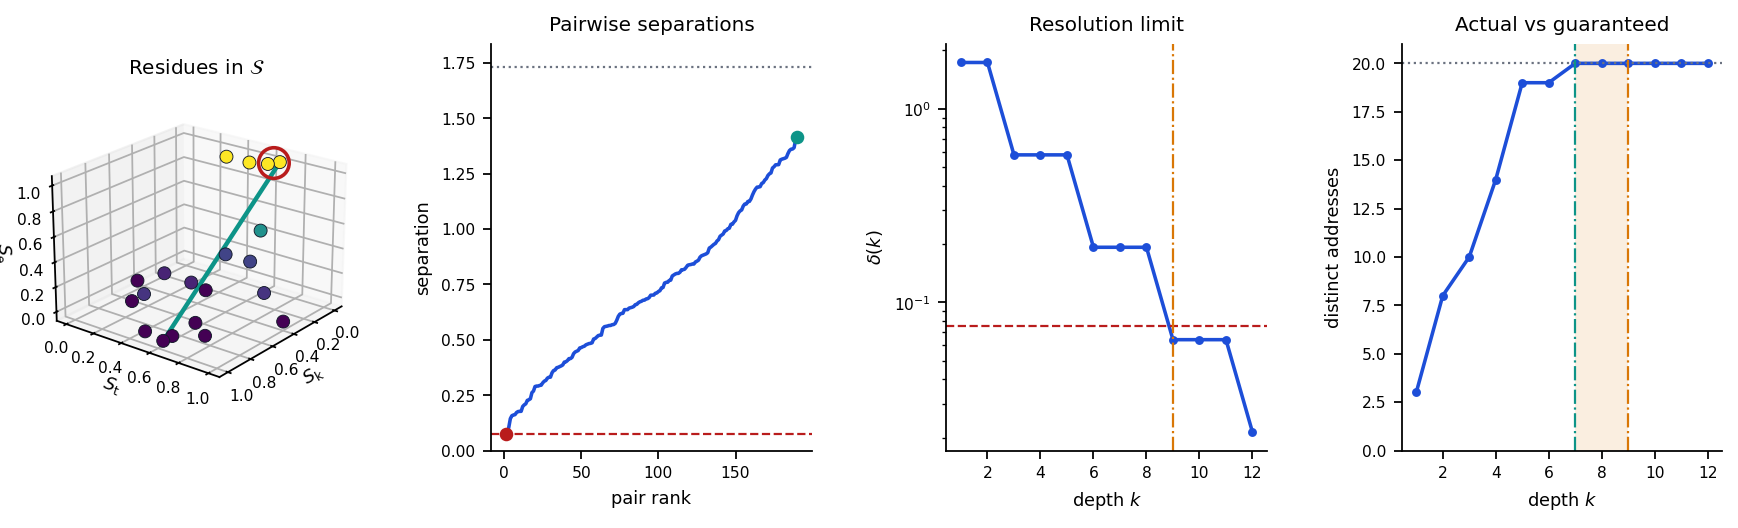
\includegraphics[width=\textwidth]{figures/panel_01_encoding.png}
\caption{\textbf{S-entropy coordinates and the resolution they force.}
(\textbf{A})~The twenty canonical residues in the S-entropy cube
$\Sspace = [0,1]^3$, coloured by $S_{\mathrm{e}}$. The teal segment is the
farthest realised pair, Ile--Arg at $d_{\max} = 1.415$; the red ring marks
Lys--Arg, the closest pair at $d_{\min} = 0.0756$, which is sub-pixel at
this scale and so is ringed rather than drawn.
(\textbf{B})~All $190$ pairwise separations in increasing order. The lower
dashed line is $d_{\min}$, the upper dotted line the cube diameter
$\sqrt3$; the curve terminates well short of it.
(\textbf{C})~The cell diagonal $\delta(k) = \sqrt3\,3^{-\lfloor k/3\rfloor}$
against $d_{\min}$. The two first meet at $k=9$, which is therefore the
guaranteed resolution depth of \Cref{thm:aa-resolution}, and the guarantee
is tight: $\delta(8) = 0.1925 > d_{\min}$.
(\textbf{D})~Addresses that are actually distinct at each depth. All twenty
separate at $k=7$ (teal), two levels below the $k=9$ guarantee (orange);
the shaded band is the slack recorded in \Cref{rem:guarantee-slack}.}
\label{fig:panel-encoding}
\end{figure*}

\begin{figure*}[!htbp]
\centering
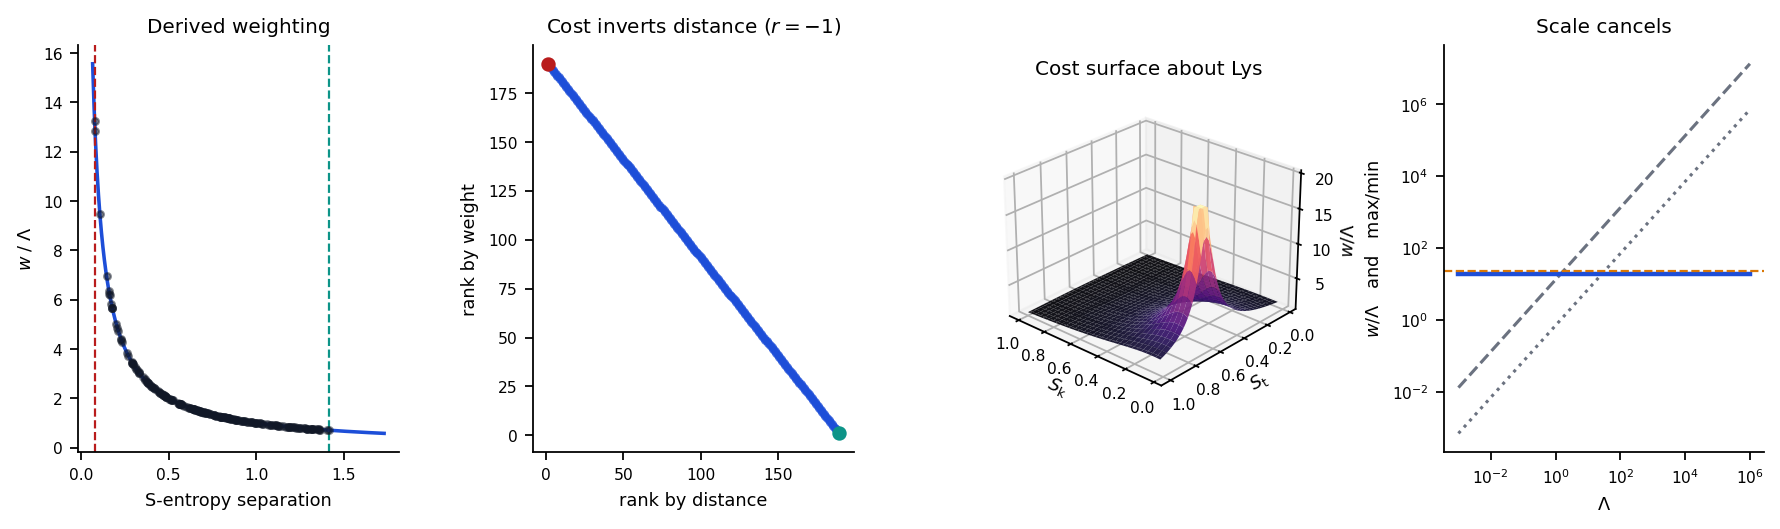
\includegraphics[width=\textwidth]{figures/panel_02_weighting.png}
\caption{\textbf{The derived contact weighting is a separation cost.}
(\textbf{A})~The weighting $\wt = \Lambda/\norm{\sse(u)-\sse(v)}$ of
\eqref{eq:wt-derived}, with the $190$ residue pairs overlaid. Dashed lines
mark $d_{\min}$ and $d_{\max}$.
(\textbf{B})~Each pair ranked independently by S-entropy distance and by
contact weight, both ascending. The rankings are exactly reversed
($r = -1$): the closest pair (red) is the most expensive to separate and
the farthest (teal) the cheapest, which is the inversion of
\Cref{rem:reciprocal} and the sense in which $\wt$ measures cost rather
than distance.
(\textbf{C})~The cost surface over an $(S_{\mathrm{k}}, S_{\mathrm{t}})$
slice through Lys, clipped at $20\Lambda$. Contact strength is a pole at
the reference residue, not a bounded similarity score.
(\textbf{D})~Individual weights (grey) sweep nine decades as $\Lambda$
varies, while their ratio (blue) does not move. The scale cancels from
every prediction, so the theory carries no fitted parameter; the orange
line is the bound $\sqrt3/d_{\min}$.}
\label{fig:panel-weighting}
\end{figure*}

\begin{figure*}[!htbp]
\centering
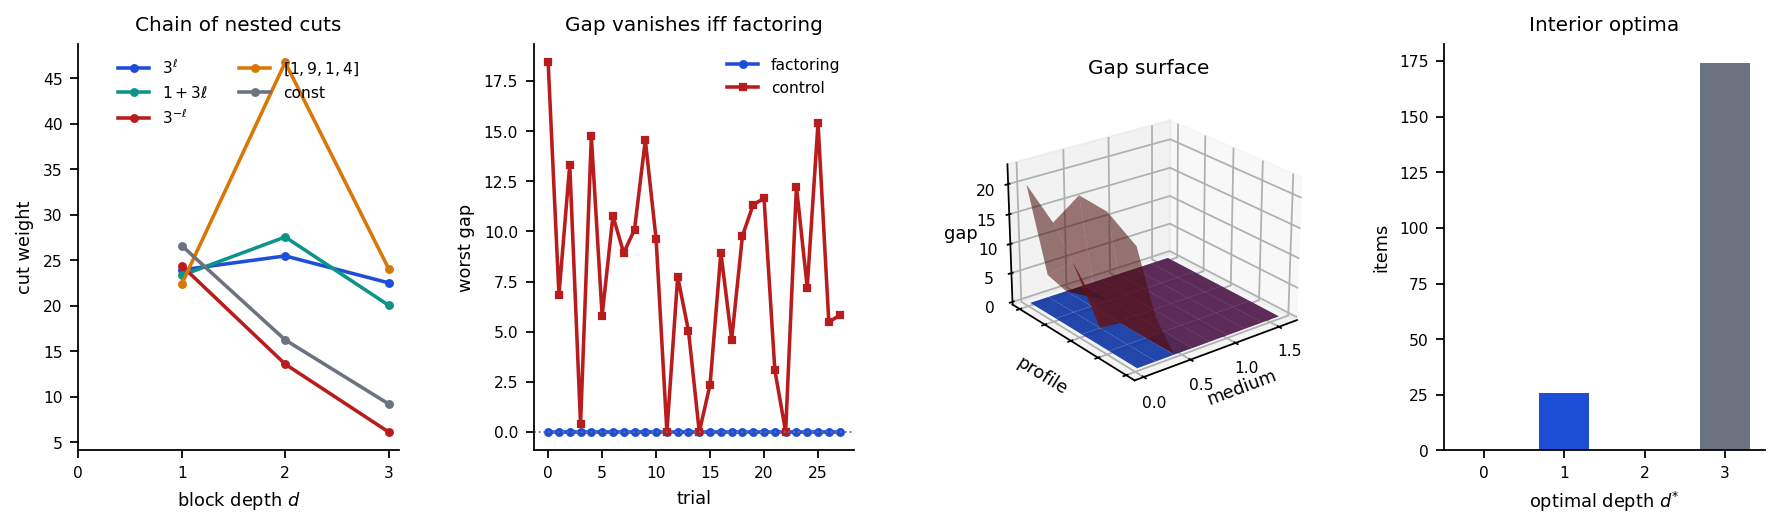
\includegraphics[width=\textwidth]{figures/panel_03_subtrie_cut.png}
\caption{\textbf{Minimum cuts land on trie boundaries, and only under the
factoring hypothesis.}
(\textbf{A})~Cut weight along the chain of nested subtrie blocks
$B_d(v)$ for five weight profiles: increasing, linear, decreasing,
non-monotone and constant. Depth $d=0$ is the degenerate whole-set cut and
is excluded throughout (\Cref{rem:degenerate-cuts}). That decreasing and
non-monotone profiles behave no differently is
\Cref{rem:factoring-not-monotone} made visible.
(\textbf{B})~The gap \eqref{eq:gap} between the chain minimum and the true
minimum over all $2^{\abs{\V}-1}$ admissible cuts. Under factoring (blue)
it is identically zero; under weights drawn independently per pair (red),
with every other feature of the instance preserved, it reaches $18.4$.
(\textbf{C})~The same contrast as a surface over medium coupling and weight
profile: the factoring sheet (blue) is flat at zero everywhere, the control
sheet (red) is not.
(\textbf{D})~Where the optimum sits. Grey bars are the two degenerate
depths, $d^{*}=0$ and $d^{*}=k$; the blue bar counts items whose optimal
block is strictly interior, confirming the result is not an artefact of the
trivial minimisers.}
\label{fig:panel-subtrie}
\end{figure*}

\begin{figure*}[!htbp]
\centering
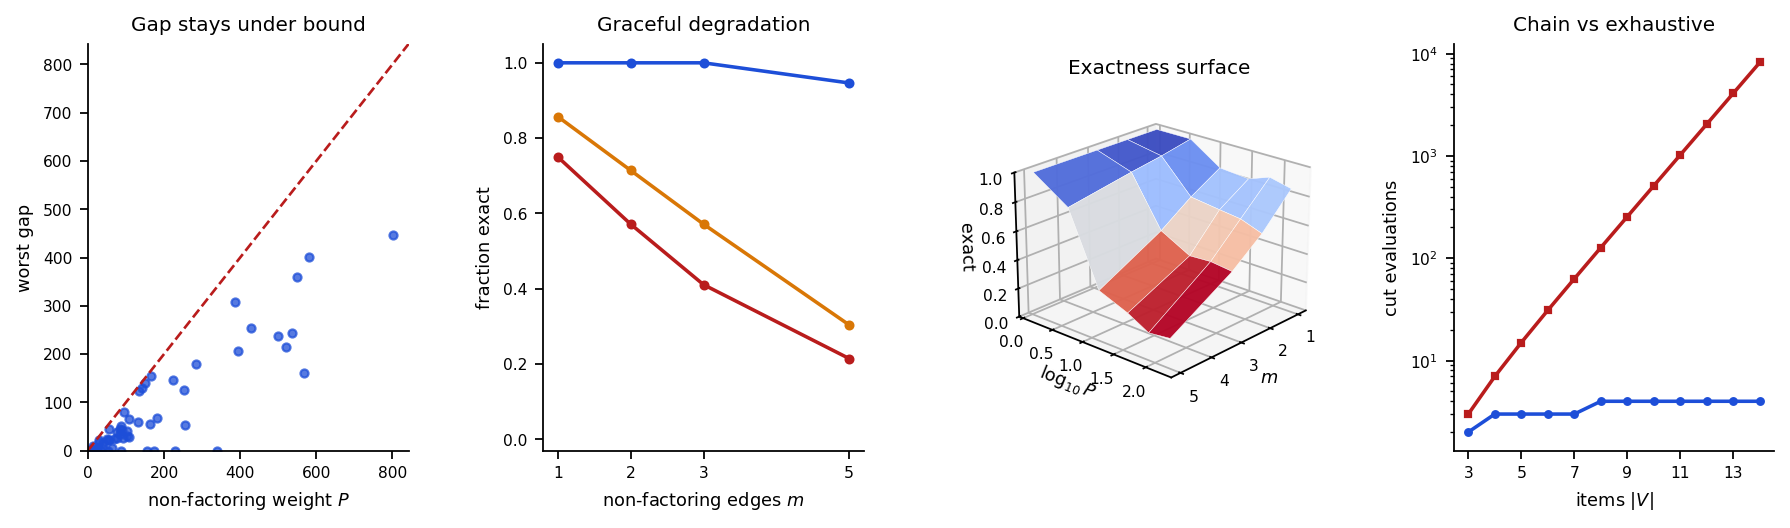
\includegraphics[width=\textwidth]{figures/panel_04_degradation.png}
\caption{\textbf{Degradation when the factoring hypothesis fails.}
Real contact graphs carry disulfides and other couplings that violate
\eqref{eq:trie-factoring}; these charts perturb a factoring graph by adding
$m$ such edges of total weight $P$.
(\textbf{A})~The gap against $P$ over all trials. Every point lies below the
identity (dashed), so the bound of \Cref{rem:complexity-honest} holds, and
points approach it closely enough ($\gapv/P$ up to $0.938$) that it is not
slack.
(\textbf{B})~Fraction of items whose separation cost is still computed
exactly, against the number of offending edges, at three perturbation
magnitudes. Degradation is monotone rather than catastrophic.
(\textbf{C})~The same quantity as a surface over $m$ and $\log_{10}P$.
Exactness falls monotonically in both directions, from unity under weak
single couplings to below $0.3$ under many strong ones.
(\textbf{D})~Cut evaluations required: $k+1$ along the chain against
$2^{\abs{\V}-1}$ exhaustively, on a logarithmic axis. This is the content
of \Cref{cor:sepcost-cheap}, counted directly rather than quoted
asymptotically.}
\label{fig:panel-degradation}
\end{figure*}

\begin{figure*}[!htbp]
\centering
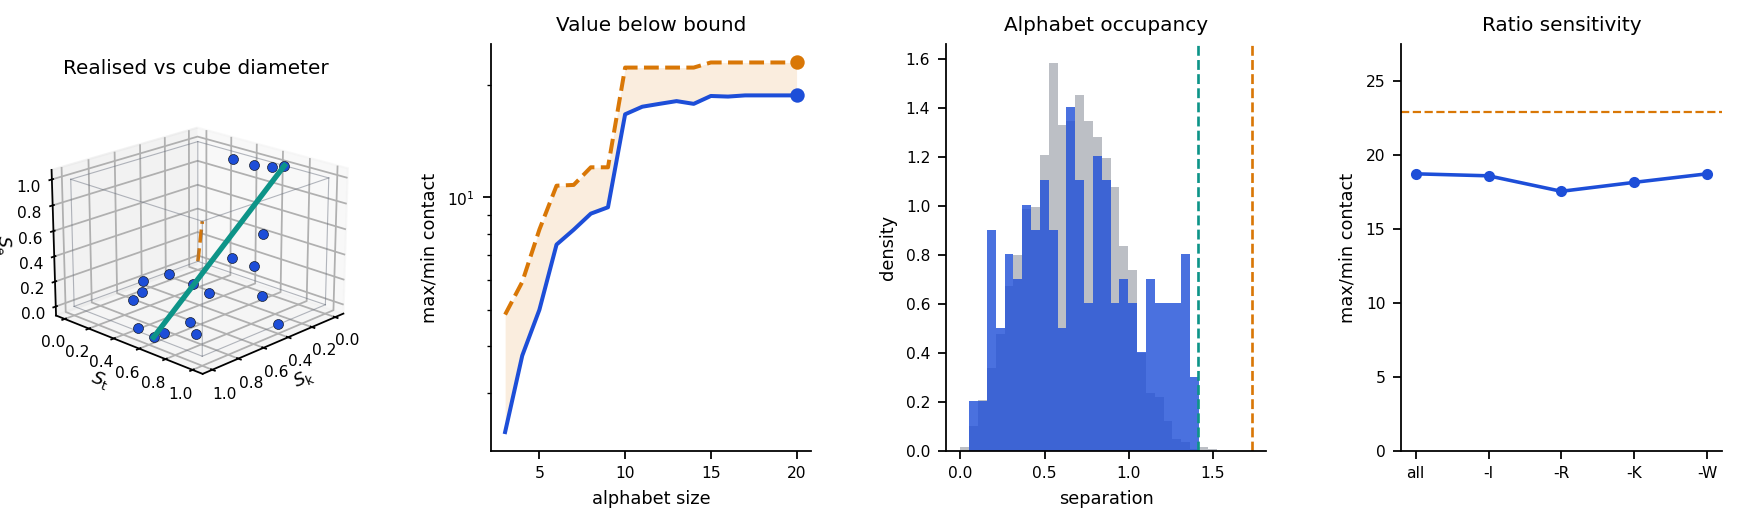
\includegraphics[width=\textwidth]{figures/panel_05_ratio.png}
\caption{\textbf{A bound distinguished from a value.}
(\textbf{A})~The residues in $\Sspace$ with the unit cube drawn. The teal
segment is the farthest realised pair, Ile--Arg; the orange dashed line is
the cube diagonal. They are not the same object, which is the whole content
of \Cref{rem:ratio-bound}: $\sqrt3$ is the diameter of the cube, and no two
residues occupy opposite corners.
(\textbf{B})~The realised contact ratio $d_{\max}/d_{\min}$ (blue) against
the bound $\sqrt3/d_{\min}$ (orange) for random sub-alphabets of increasing
size. The shaded band between them is the overstatement the validation
caught; it narrows as the alphabet fills the cube, closing at $18.7$
against $22.9$ for the full twenty.
(\textbf{C})~Distribution of residue separations (blue) against separations
between uniformly random points of the cube (grey). The alphabet reaches
$82\%$ of the available diameter --- spread through $\Sspace$, but not to
its extremes (\Cref{rem:alphabet-occupancy}).
(\textbf{D})~Sensitivity of the ratio to removing each residue of the
extreme pairs. It moves by less than $7\%$, so $18.7$ is a property of the
alphabet rather than of one outlying pair.}
\label{fig:panel-ratio}
\end{figure*}


% =====================================================================
% Bibliography
% =====================================================================
ibliographystyle{plainnat}
ibliography{references}

\end{document}
